\documentclass[conference]{IEEEtran}
\IEEEoverridecommandlockouts
\usepackage{cite}
\usepackage{amsmath,amssymb,amsfonts}
\usepackage{algorithmic}
\usepackage{graphicx}
\usepackage{textcomp}
\usepackage{xcolor}
\usepackage{float}
\usepackage{rotating}

\def\BibTeX{{\rm B\kern-.05em{\sc i\kern-.025em b}\kern-.08em
    T\kern-.1667em\lower.7ex\hbox{E}\kern-.125emX}}

\begin{document}
\sloppy

\title{AquaOptima: Apply Evolutionary Algorithm and Particle Swarm Optimization in Virtual Largemouth Bass Aquaculture\\}

\author{
\IEEEauthorblockN{Leon Hoang}
\IEEEauthorblockA{\textit{Tickle College of Engineering} \\
University of Tennessee, Knoxville\\
Knoxville, TN\\
phoang5@vols.utk.edu}
\and
\IEEEauthorblockN{Ahmed Ghazi}
\IEEEauthorblockA{\textit{Tickle College of Engineering} \\
University of Tennessee, Knoxville\\
Knoxville, TN\\
aghazi2@vols.utk.edu}
}

\maketitle

\begin{abstract}
\normalfont
This report investigates the optimization of Largemouth Bass (\textit{Micropterus salmoides}) aquaculture policies using a custom biologically-inspired simulation, AquaOptima. The project addresses the critical challenge of maintaining high survival rates and optimal fish health while minimizing economic cost. AquaOptima employs Particle Swarm Optimization (PSO) to create a biologically realistic 3D agent-based model of fish behavior, capturing complex dynamics such as foraging, oxygen-seeking, disease avoidance, and intracohort cannibalism. To discover optimal management strategies, an Evolutionary Algorithm (EA) evaluates and mutates policies governing food, probiotic, and oxygen distribution. Across 10 separate timelines and 20 generations, the EA successfully navigated the exploration-exploitation tradeoff, converging on policies that eliminate starvation and suffocation without exceeding strict budgetary constraints. Ultimately, the results demonstrate the efficiency of combining PSO led agent models with evolutionary algorithms to reliably solve multi-objective physical phenomena in modern aquaculture systems.
\end{abstract}

\begin{IEEEkeywords}
Particle Swarm Optimization, Evolutionary Algorithms, Agent-Based Modeling, Aquaculture, Micropterus salmoides
\end{IEEEkeywords}

\section{Introduction and Motivation}

\subsection{Project Goal}
Aquaculture operations face constant pressure to maximize yield while adhering to strict economic and environmental constraints. The overarching goal of this project is to develop an intelligent, automated management system capable of optimizing resource distribution, specifically food, probiotics, and oxygen, for Largemouth Bass.

\subsection{Research Question}
The primary research question addressed in this paper is: Can Evolutionary Algorithms (EA) be used to optimize the parameters of a complex, agent-based model (driven by Particle Swarm Optimization) to maximize the survival and health of a simulated fish population while minimizing operational costs?

\subsection{Topic Significance and Algorithm Selection}
This topic is of particular interest because biological systems are highly sensitive to environmental factors. Largemouth Bass populations are prone to high mortality rates during summer seasons, are highly susceptible to bacterial pathogens, and exhibit natural intracohort cannibalism when starved. Standard mathematical models often fail to capture these localized, agent-level interactions. By utilizing bio-inspired computation, especially PSO to simulate the swarm intelligence of the fish and EA to evolve the management policies, we can realistically simulate these physical phenomena and derive highly optimized, non-intuitive solutions that traditional optimization methods might miss.

\section{Related Work}
Agent-based modeling (ABM) and bio-inspired algorithms are increasingly utilized to understand complex biological systems. Previous works have established the efficiency of using ABM in fisheries and aquaculture, successfully simulating factors like dissolved oxygen levels, fish shoal behavior, and spatial management strategies \cite{carrella2024}, \cite{urbanova2023}.

In the specific context of Largemouth Bass aquaculture, researchers have documented the severe environmental impacts of poor pond management in maintaining survival rates \cite{hou2023}. Disease management remains a massive hurdle, with extensive research dedicated to controlling mortality caused by bacterial pathogens like \textit{Columnaris} and \textit{Aeromonas} \cite{bowker2013}, \cite{tu2025}. To combat this, recent studies have proven the effectiveness of dietary probiotic supplementation (such as \textit{Lactobacillus reuteri}) to significantly boost fish immunity and metabolism \cite{wang2024}. Furthermore, behavioral constraints, such as aggressive intracohort cannibalism driven by size disparity and starvation, are well-documented phenomena in Age-0 Largemouth Bass \cite{johnson1996}.

Computationally, Particle Swarm Optimization (PSO) has been a foundational bio-inspired algorithm since its introduction, modeling the social behavior of bird flocks and fish schools to optimize non-linear functions \cite{kennedy1995}. However, while existing research applies ABMs to observe fish, and uses PSO for general mathematical optimization, few studies bridge the gap.

What AquaOptima does differently is that it directly integrates biological reality with computational optimization. Instead of treating the fish as static data points, this project uses a modified PSO algorithm to simulate real-time survival behaviors (schooling, fleeing hazards, foraging). It then wraps this highly volatile simulation in an EA to evolve an external manager policy.

\section{Experimental Setup and Approach}
The experiment was constructed entirely within a custom Python simulation. The simulation relies on two distinct biologically-inspired algorithms operating together.

\subsection{The Environment}
The simulation takes place in a 3D pond space with dimensions of $180 \times 85 \times 50$ (width $\times$ height $\times$ depth). To establish a biologically realistic population, the initial fish count (finalized at 50 fish) is calculated dynamically based on the pond's volume using a density scaling factor ($K = 0.55$) derived from standard intensive pond culture guidelines \cite{tidwell1998}:
\begin{equation}
\boxed{
InitialFish = \max\left(10, \left\lfloor K \times (W \times H \times D)^{\frac{1}{3}} \right\rfloor\right)
}
\end{equation}

Also, the environment operates on a complex, cyclic interaction model where physical objects and biological agents continuously influence each other:
\begin{itemize}
    \item \textbf{Consumption and Waste:} Fish consume dropped food, probiotics, and oxygen bubbles to replenish their physiological stats. As fish metabolize, they routinely produce sinking fecal waste, a primary driver of pond eutrophication \cite{hou2023}.
    \item \textbf{Pollutant Transformation:} Uneaten food, expired probiotics, and accumulated fecal waste on the pond floor eventually decay into generic pollutants. Over time, these pollutants likely transform into environmental hazards.
    \item \textbf{Environmental Hazards:} Water quality degradation introduces severe physiological penalties \cite{hou2023}. Ammonia (NH3) hazards deplete fish oxygen and health by restricting respiratory efficiency. Furthermore, disease and parasite zones severely drain fish immunity and induce long-term physiological decay \cite{bowker2013}, \cite{tu2025}.
    \item \textbf{Mortality:} If a fish starves, suffocates, or succumbs to disease, its body will either sink or float. These decaying bodies act as massive, localized ammonia emitters before ultimately breaking down into dense pollutants, creating a deadly feedback loop in crowded spaces \cite{hou2023}, \cite{bowker2013}.
    \item \textbf{Cannibalism:} Largemouth Bass was intentionally selected for its aggressive intracohort cannibalism \cite{johnson1996}. This creates a complex predator-prey dynamic, where starved fish target smaller cohort members, without the computational overhead of additional predatory species. Successful cannibalism immediately removes the target while providing substantial fullness for the predator.
\end{itemize}
\subsection{PSO Agent Behavior}
The fish agents are driven by a modified PSO velocity update algorithm. Rather than seeking a single mathematical global minimum, each particle's (fish's) velocity vector is influenced by a dynamic weighting system based on its internal physiological state:

\begin{table}[htbp]
\centering
\caption{PSO Behavioral Weight Parameters}
\label{tab:pso_params}
\begin{tabular}{|l|c|l|}
\hline
\textbf{Parameter} & \textbf{Base Weight} & \textbf{Behavior} \\ \hline
${\text{cFood}}$      & 3x   & Toward nearest food source \\ \hline
${\text{cOxygen}}$    & 2x   & Toward nearest oxygen bubble \\ \hline
${\text{cSelfish}}$   & 1.5x & Away from nearest fish \\ \hline
${\text{cDisease}}$   & 2.5x & Away from nearest disease area \\ \hline
${\text{cObstacle}}$  & 2x   & Away from nearest obstacle \\ \hline
${\text{cRun}}$       & 5x   & Away from nearest larger fish \\ \hline
${\text{cProbiotic}}$ & 1.5x & Toward nearest probiotic \\ \hline
${\text{cSocial}}$    & 1.5x & Toward global optima (schooling) \\ \hline
${\text{cNH3}}$       & 4x   & Away from nearest ammonia zone \\ \hline
${\text{cParasite}}$  & 3x   & Away from nearest parasite area \\ \hline
${\text{cWander}}$    & 1x   & Toward pond center when isolated \\ \hline
\end{tabular}
\end{table}

These twelve parameters collectively define four behavioral modes:

\begin{itemize}
    \item \textbf{Foraging and Supplementation:} ${\text{Food}}$ (3x) is the 
    driving force under normal conditions, steering particles toward the nearest food 
    pellet with the urgency scaling with lower
    fullness levels. ${\text{Probiotic}}$ (1.5x) similarly draws fish toward probiotic 
    pellets, but only activates when immunity drops below 100\%, making it a conditional behavior.

    \item \textbf{Physiological Survival:} ${\text{Oxygen}}$ (2x) activates when a 
    fish's dissolved oxygen reserve falls below the 70\% threshold, overriding 
    lower priority behaviors to steer the fish toward the nearest oxygen bubble. 
    ${\text{Wander}}$ (1x) serves as a fallback, which directs isolated fish 
    with no nearby neighbors back toward the pond center to maintain loose schooling behavior.

    \item \textbf{Hazard Avoidance:} This mode contains the highest-weight parameters 
    in the system. ${\text{Run}}$ (5x) is the single strongest behavioral force, 
    driving fish to flee from any detected larger mouthed fish to avoid 
    intracohort cannibalism. ${\text{NH3}}$ (4x) manages ammonia exposure. NH3 repels fish from poisonous
    zones${\text{Disease}}$ (2.5x) and ${\text{Parasite}}$ (3x) 
    provide directional repulsion from each of their hazard zones. 
    ${\text{Obstacle}}$ (2x) prevents fish from clipping into solid boundaries.

    \item \textbf{Schooling:} Standard PSO social dynamics are preserved through 
    ${\text{Selfish}}$ (1.5x) and ${\text{Social}}$ (1.5x), which implement 
    separation and global best attraction forces, which balances individual 
    spacing against group cohesion and prevents clustering in 
    resource dense areas.
\end{itemize}

The relative magnitudes of these weights encode a biologically-motivated priority 
hierarchy: predator evasion and toxin avoidance are prioritized over foraging, which is prioritized over 
social schooling. This hierarchy ensures that when multiple parameters compete 
simultaneously, the most prioritized behavior 
reflects realistic survival instincts rather than resource seeking.
\subsection{Evolutionary Algorithm (EA) Setup}
The EA functions as an "Aquaculture Grower," which is responsible for sustaining the PSO fish swarm. Biological reproduction is omitted to limit computational complexity. Instead, the evolutionary process optimizes controllable aquaculture policies rather than the stochastic biological and physical dynamics of the pond. To accurately model and optimize this environment, the EA was structured with the following components:

\subsubsection{Parameters}
To ensure robust evaluation and statistical significance, the experiment parameters are defined as follows:
\begin{itemize}
    \item \textbf{Timelines:} 10 independent timelines. The variance between timelines is driven by two factors: the randomized genotypes of the initial populations, and the chaotic outcomes stemming from the stochastic nature of the environment setup.
    \item \textbf{Generations:} 20 generations per timeline.
    \item \textbf{Population Size:} 20 candidate policies per generation.
    \item \textbf{Simulation Duration:} 30-day aquaculture period, where each time step represents 1 hour in the virtual simulation.
    \item \textbf{Budget Constraint:} Strict maximum budget of \$500. If a policy exhausts this budget before day 30, the simulation terminates early for that pond.
    \item \textbf{Resource Costs:} Food at \$0.10 per pellet, Probiotics at \$0.50 per pellet, and Oxygen pumping at \$1.50 per duration hour.
\end{itemize}

\subsubsection{Genotype}
The genotype represents a specific aquaculture policy consisting of 9 parameters, detailed in Table \ref{tab:genotype}.

\begin{table}[htbp]
\centering
\caption{Genotype Parameters, Ranges, and Mutations}
\label{tab:genotype}
\begin{tabular}{|p{0.25\linewidth}|p{0.65\linewidth}|}
\hline
\textbf{Resource} & \textbf{Parameters (Range) [Mutation Step]} \\ \hline
\textbf{Food} & Interval: 1--24h [$\pm$4h] \newline Quantity: 1--10 pellets [$\pm$2] \newline Location: Center or Random [Flip] \\ \hline
\textbf{Probiotics} & Interval: 12--168h [$\pm$1 index] \newline Quantity: 0--4 pellets [$\pm$1] \newline Location: Center or Random [Flip] \\ \hline
\textbf{Oxygen} & Interval: 1--24h [$\pm$4h] \newline Duration: 1--3h [$\pm$1h] \newline Location: Center or Random [Flip] \\ \hline
\end{tabular}
\end{table}

The EA utilizes an 80\% ($0.80$) crossover rate to recombine successful traits within the stochastic environment, balanced by a 25\% ($0.25$) mutation rate to prevent premature convergence. Mutation applies binary flips for categorical drop locations and Gaussian perturbation for numeric parameters. By taking small, localized steps (e.g., slightly shifting a 12-hour interval to 16 hours), Gaussian perturbation enables safe fine-tuning of near-optimal solutions without causing destructive, erratic deviations from elite policies \cite{hinterding1995}.

\subsubsection{Fitness Function}
The fitness function acts as the mathematical compass for the evolutionary algorithm, driving the swarm towards optimal multi-objective performance. The function automatically rejects any policy that exceeds the strict \$500 operational budget. For policies within the budget, it aggregates three normalized metrics (scaled from 0 to 1) into a single scalar value:

\begin{equation}
\boxed{
\begin{aligned}
Fitness ={} & 0.55 \times SurvivalRate \\
            & + 0.33 \times SavingRate \\
            & + 0.12 \times Healthiness
\end{aligned}
}
\end{equation}

Each term was explicitly weighted to reflect real-world aquaculture priorities:
\begin{itemize}
    \item \textbf{SurvivalRate (0.55):} The highest priority. It is calculated as the final percentage of the original fish population still alive at day 30. Keeping the population alive is the absolute prerequisite for any viable aquaculture business.
    \item \textbf{SavingRate (0.33):} The second priority. Calculated as the fraction of the \$500 budget remaining at the end of the simulation. This incentivizes the algorithm to find minimal-resource strategies rather than continually dumping expensive food and oxygen into the pond.
    \item \textbf{Healthiness (0.12):} The final priority. It measures the aggregate average internal physiological state of the surviving fish (e.g., immunity levels, starvation levels). This acts as a tie-breaker, ensuring that between two policies with equal survival and cost, the EA prefers the one where the fish are in better physical condition.
\end{itemize}

The fitness function reflects optimization frameworks that concurrently balance growth, energy usage, and stress welfare \cite{wang2025}. This weighting mandates that the EA systematically reconcile biological welfare with economic viability.

\subsubsection{Selection and Verification}
Because the PSO simulation is highly stochastic (fish movements, random hazard spawns), evaluating a policy is partly random. A policy might score well purely by chance. To mitigate this without adding excessive computational overhead, the EA employs a selection mechanism:
\begin{itemize}
    \item \textbf{Elitism:} The top performers are automatically preserved with a rate of $k = 10\%$ of the population (which equates to $k = 2$ given the population size of 20).
    \item \textbf{Tournament Selection:} The remaining population is generated via tournament selection with a tournament size of $k = 50\%$ of the population (which equates to $k=10$ given the population size of 20).
    \item \textbf{Wilcoxon Rank-Sum Verification:} To mitigate environmental noise and stochastic luck, a cascade verification system utilizes non-parametric Wilcoxon rank-sum tests ($\alpha = 0.05$) to establish statistical dominance \cite{derrac2011}. Both the champion and challenger require a minimum of three independent simulation samples before evaluation. If the test results are unclear, the system advances through a cascade of up to three challengers, ensuring that tournament winners are superior while minimizing computational overhead. 
\end{itemize}

\section{Results}

The following plots detail policy convergence and performance metrics across 10 independent timelines, a setup designed to reduce environmental noise. Subsequent analysis focuses on the underlying biological and economic implications rather than visual trends.

\begin{figure}[H]
\centering
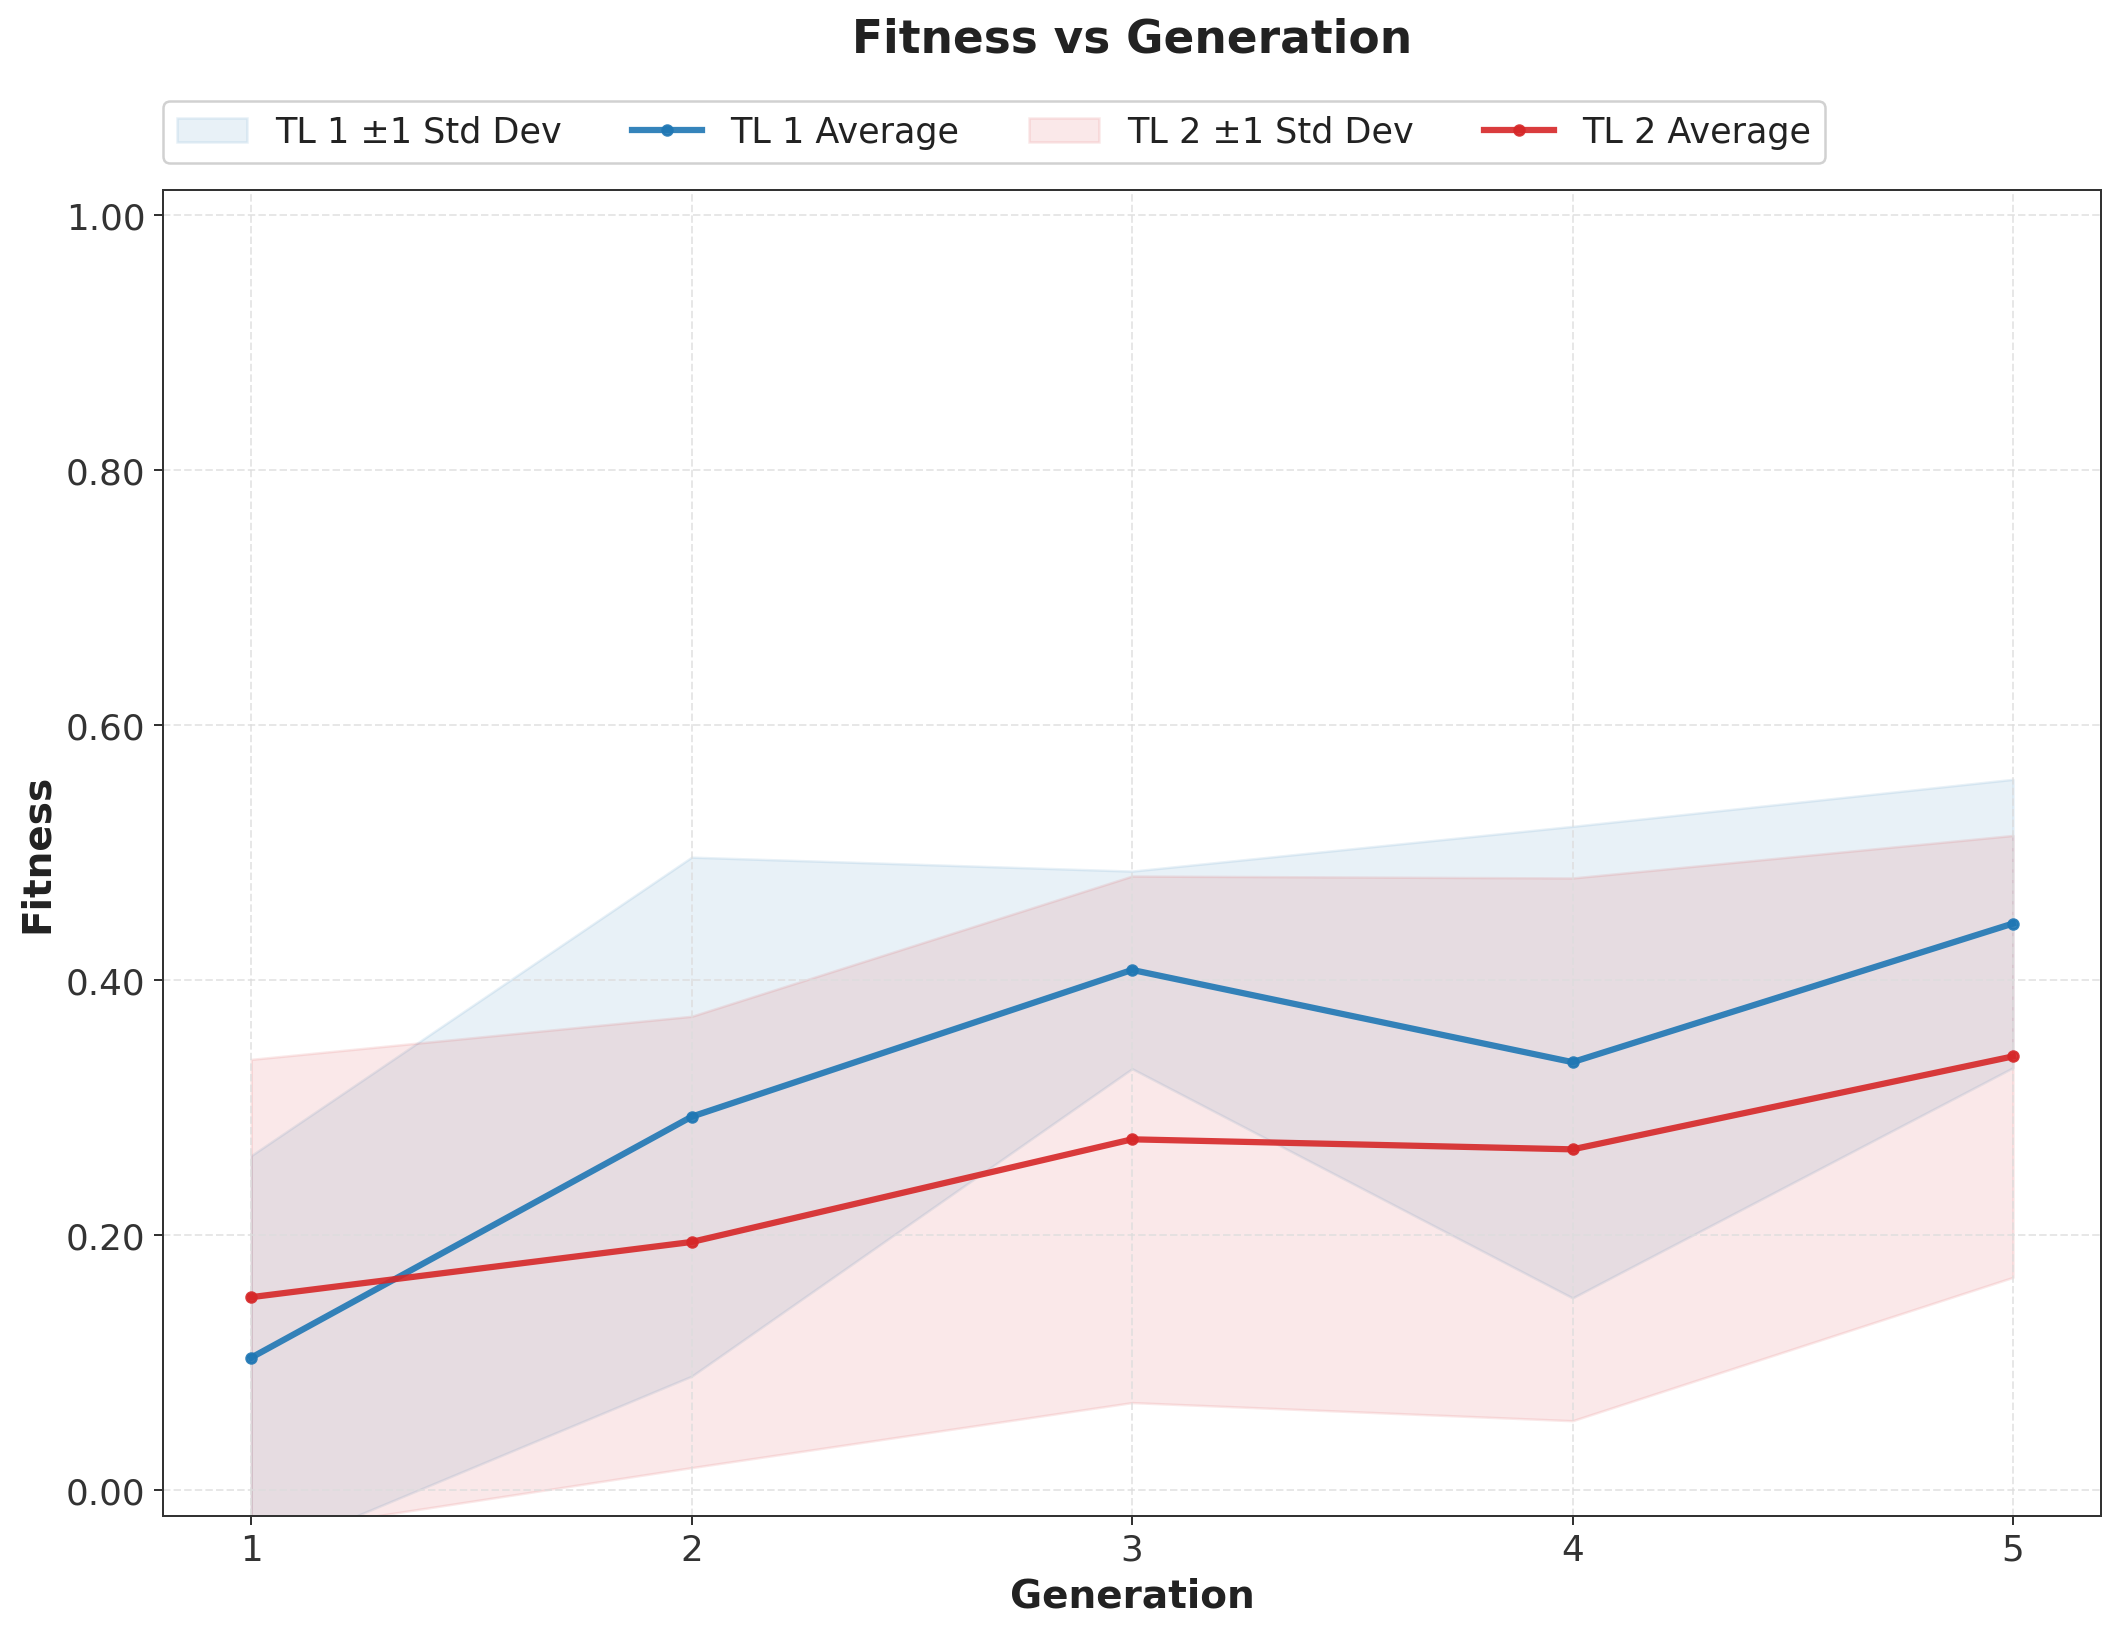
\includegraphics[width=0.42\textwidth]{../plots/plot_01_fitness_vs_gen.png}
\caption{Fitness vs Generation}
\label{fig:fitness_gen}
\end{figure}

As shown in Fig. \ref{fig:fitness_gen}, despite initial stochasticity and widespread failure in early generations, the EA successfully and consistently drives the swarm toward optimal management policies across all independent runs. Notably, the fitness score converges and fluctuates around 0.7, with the absolute best elite policies peaking near 0.8, rather than climbing to a perfect 1.0. This plateau is an intentional feature of the multi-objective fitness function. Survival Rate and Saving Rate are competing factors: keeping more fish alive inherently requires spending more money on resources. The only theoretical way to achieve a perfect 1.0 fitness score would be to achieve 100\% survival while spending absolutely zero dollars. Because that is a biological and economic impossibility, the true target of the EA is to find the optimal point (around 0.7) where biological welfare and financial efficiency are perfectly balanced, rather than chasing an impossible perfect score.


\begin{figure}[H]
\centering
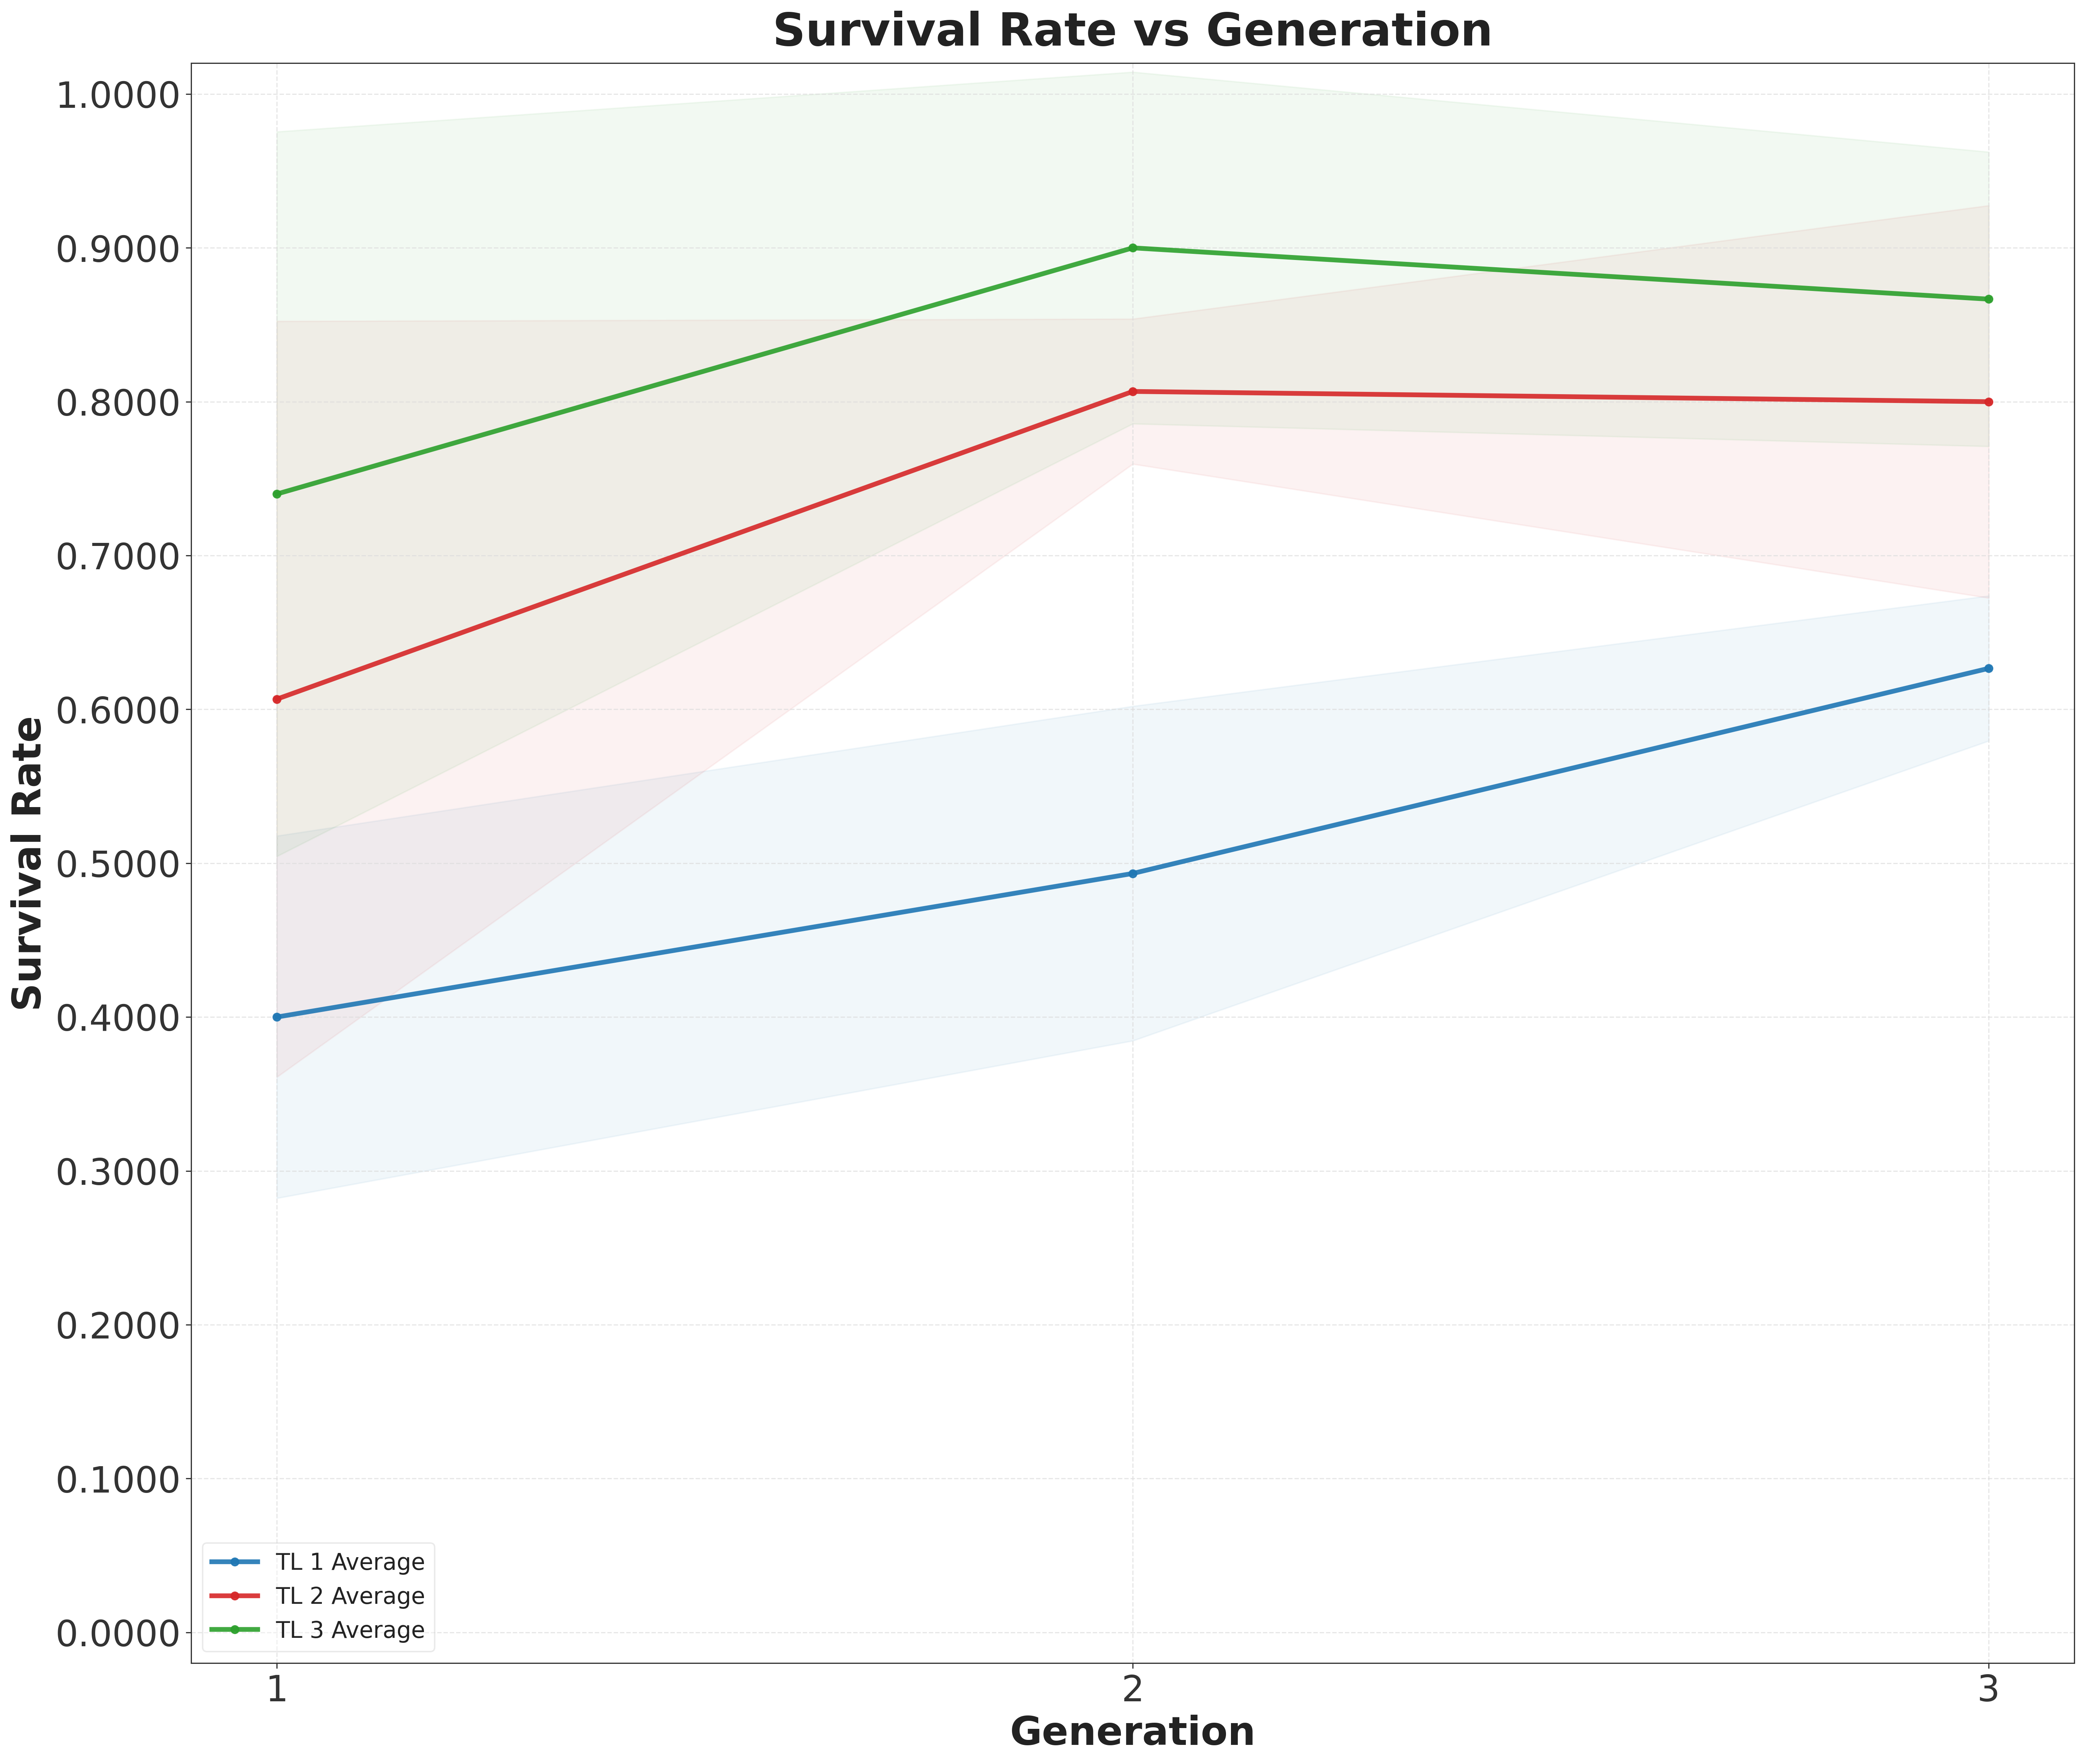
\includegraphics[width=0.42\textwidth]{../plots/plot_02_survival_rate_vs_gen.png}
\caption{Survival Rate vs Generation}
\label{fig:surv_gen}
\end{figure}

As depicted in Fig. \ref{fig:surv_gen}, the Survival Rate exhibits the most dramatic improvement among all metrics, climbing rapidly from an initial average near 0.2 up to a stable convergence around 0.8. Because Survival Rate is the most heavily weighted component of the fitness function ($0.55$), the EA aggressively optimizes for it first. The data indicates that in the chaotic virtual ponds and early random policies lead to massive population wipeouts. However, within just 5 to 7 generations, the algorithm successfully discovers and propagates foundational policies that keep the majority of the swarm alive through the full 30 day cycle.


\begin{figure}[H]
\centering
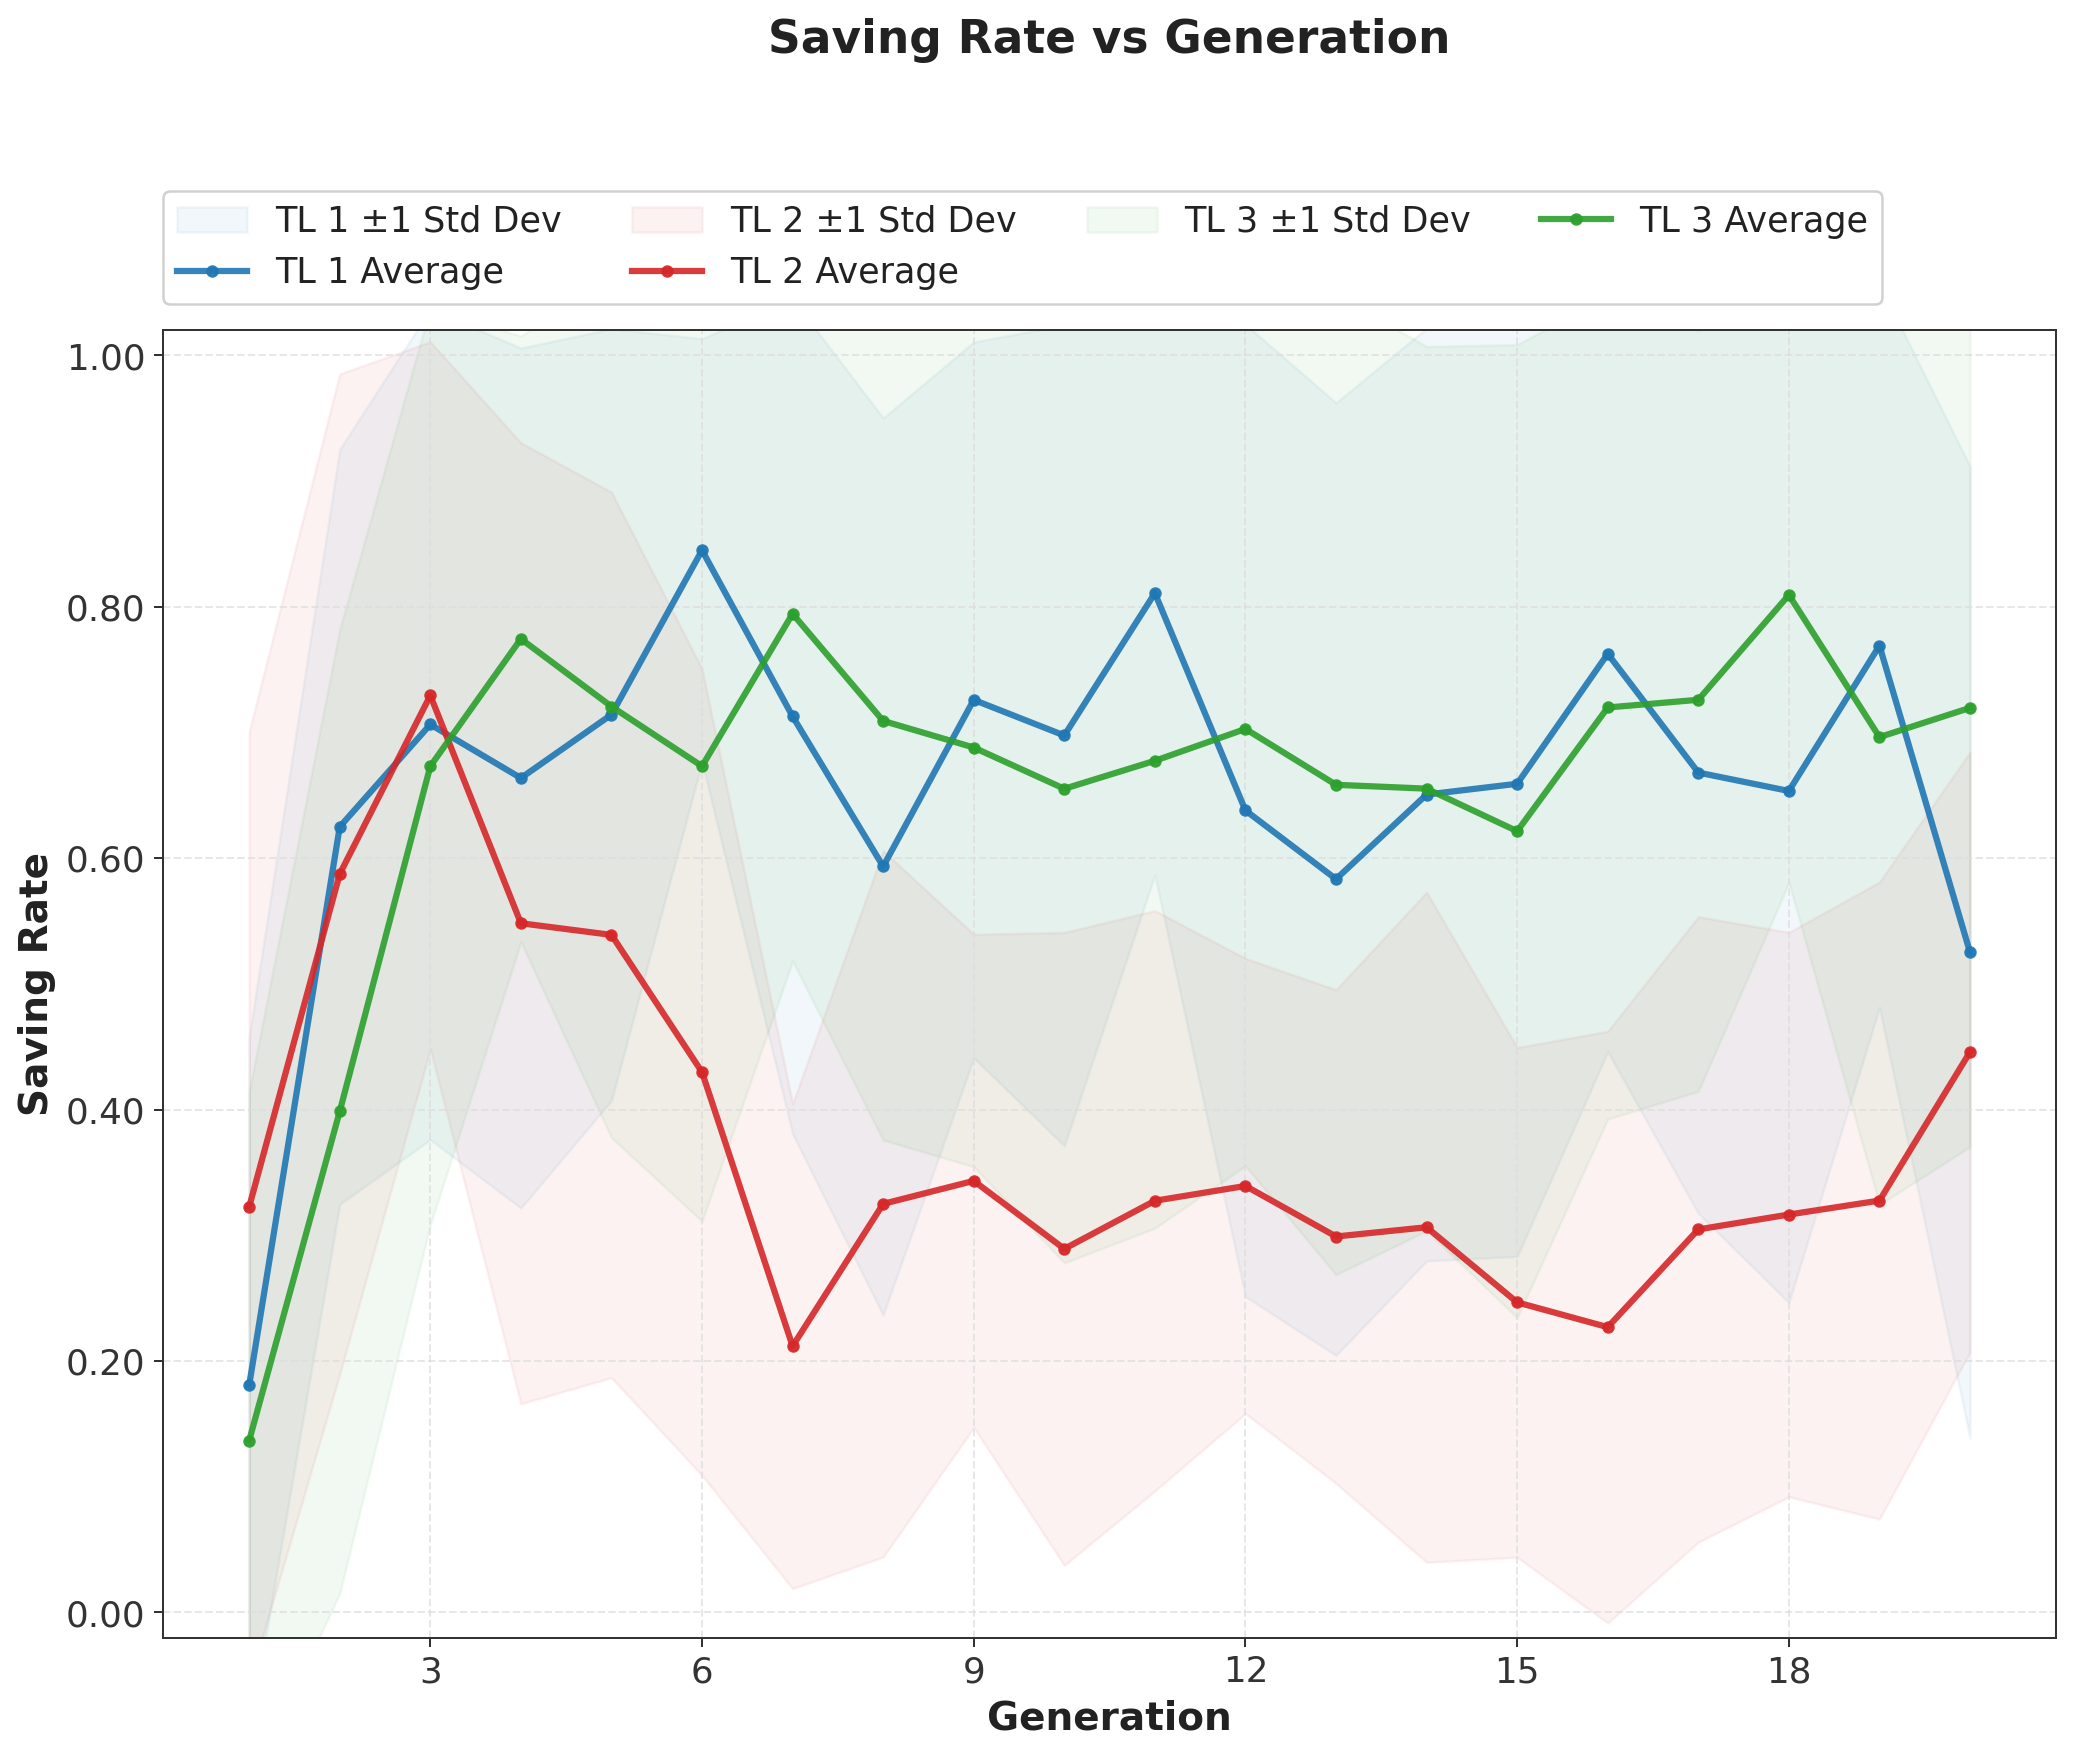
\includegraphics[width=0.42\textwidth]{../plots/plot_03_saving_rate_vs_gen.png}
\caption{Saving Rate vs Generation}
\label{fig:saving_gen}
\end{figure}

Fig. \ref{fig:saving_gen} illustrates the evolutionary trajectory of the Saving Rate. Unlike the rapid climb of the Survival Rate, the Saving Rate experiences a slight initial dip before slowly recovering and stabilizing around 0.6. This curve perfectly captures the cost of learning. In early generations, the EA attempts to maximize survival by over-allocating resources by dumping excessive food and oxygen into the pond to prevent fish death. Once the swarm achieves a stable survival baseline, the algorithm begins to refine the policies, stripping away excess resource expenditures to optimize the secondary Saving Rate metric without triggering starvation.


\begin{figure}[H]
\centering
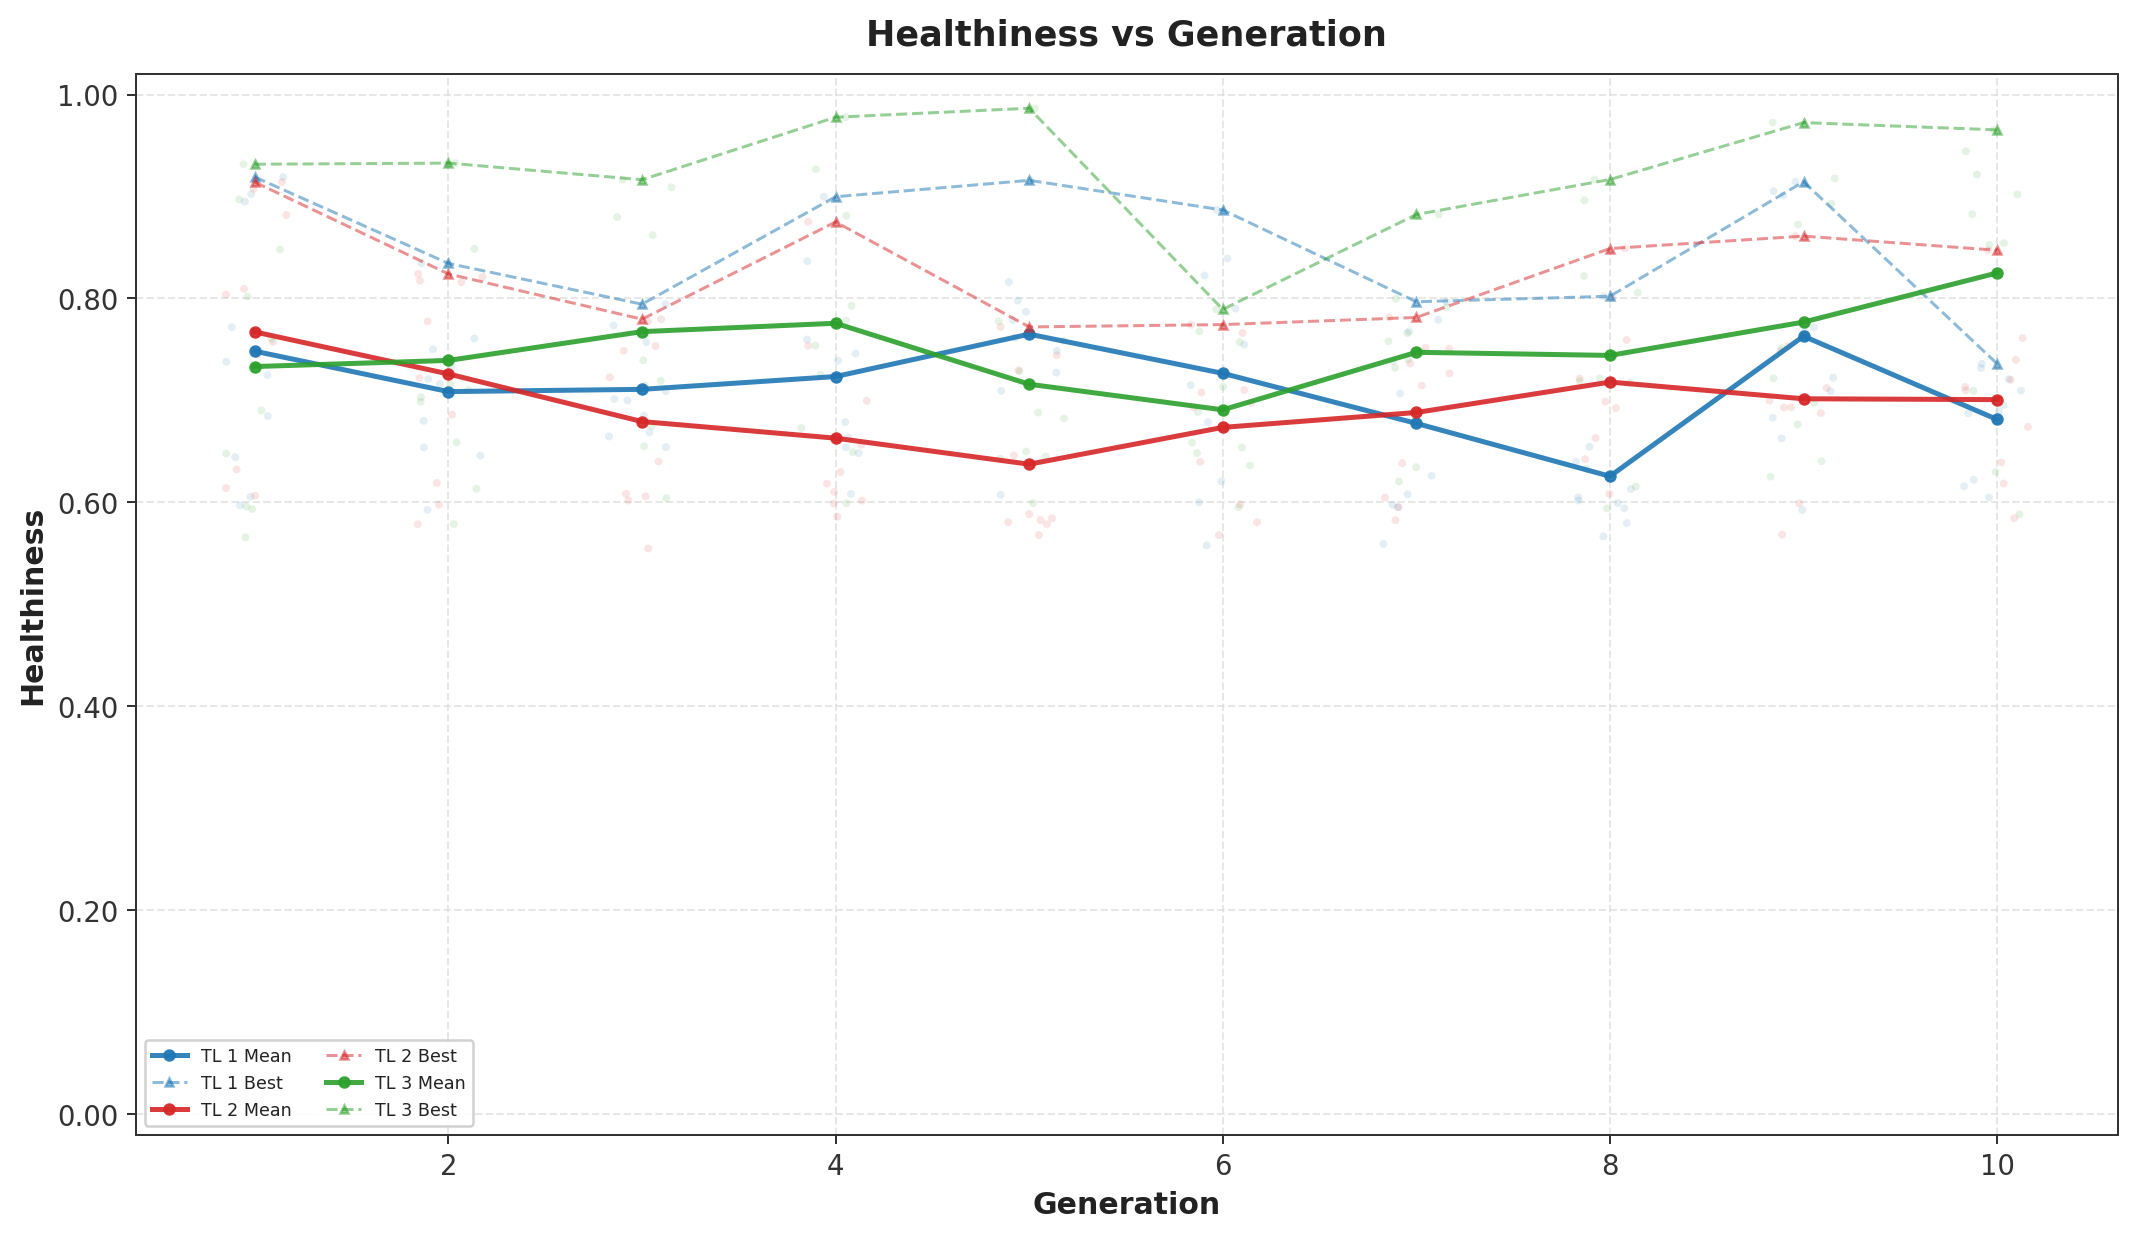
\includegraphics[width=0.42\textwidth]{../plots/plot_04_healthiness_vs_gen.png}
\caption{Healthiness vs Generation}
\label{fig:health_gen}
\end{figure}

Fig. \ref{fig:health_gen} maps the Healthiness metric across the generations. This metric converges to a relatively high baseline (between 0.7 and 0.8) very quickly. Because Healthiness is intrinsically tied to survival, a fish cannot survive the 30-day simulation if its health drops to zero. Any policy that manages to achieve a high Survival Rate naturally results in a surviving population with an acceptable health baseline. Since it carries the lowest weight ($0.12$) in the fitness function, it acts strictly as a fine-tuning tie-breaker in later generations, ensuring that surviving fish are not left in a perpetually starved or diseased state.


\begin{figure}[H]
\centering
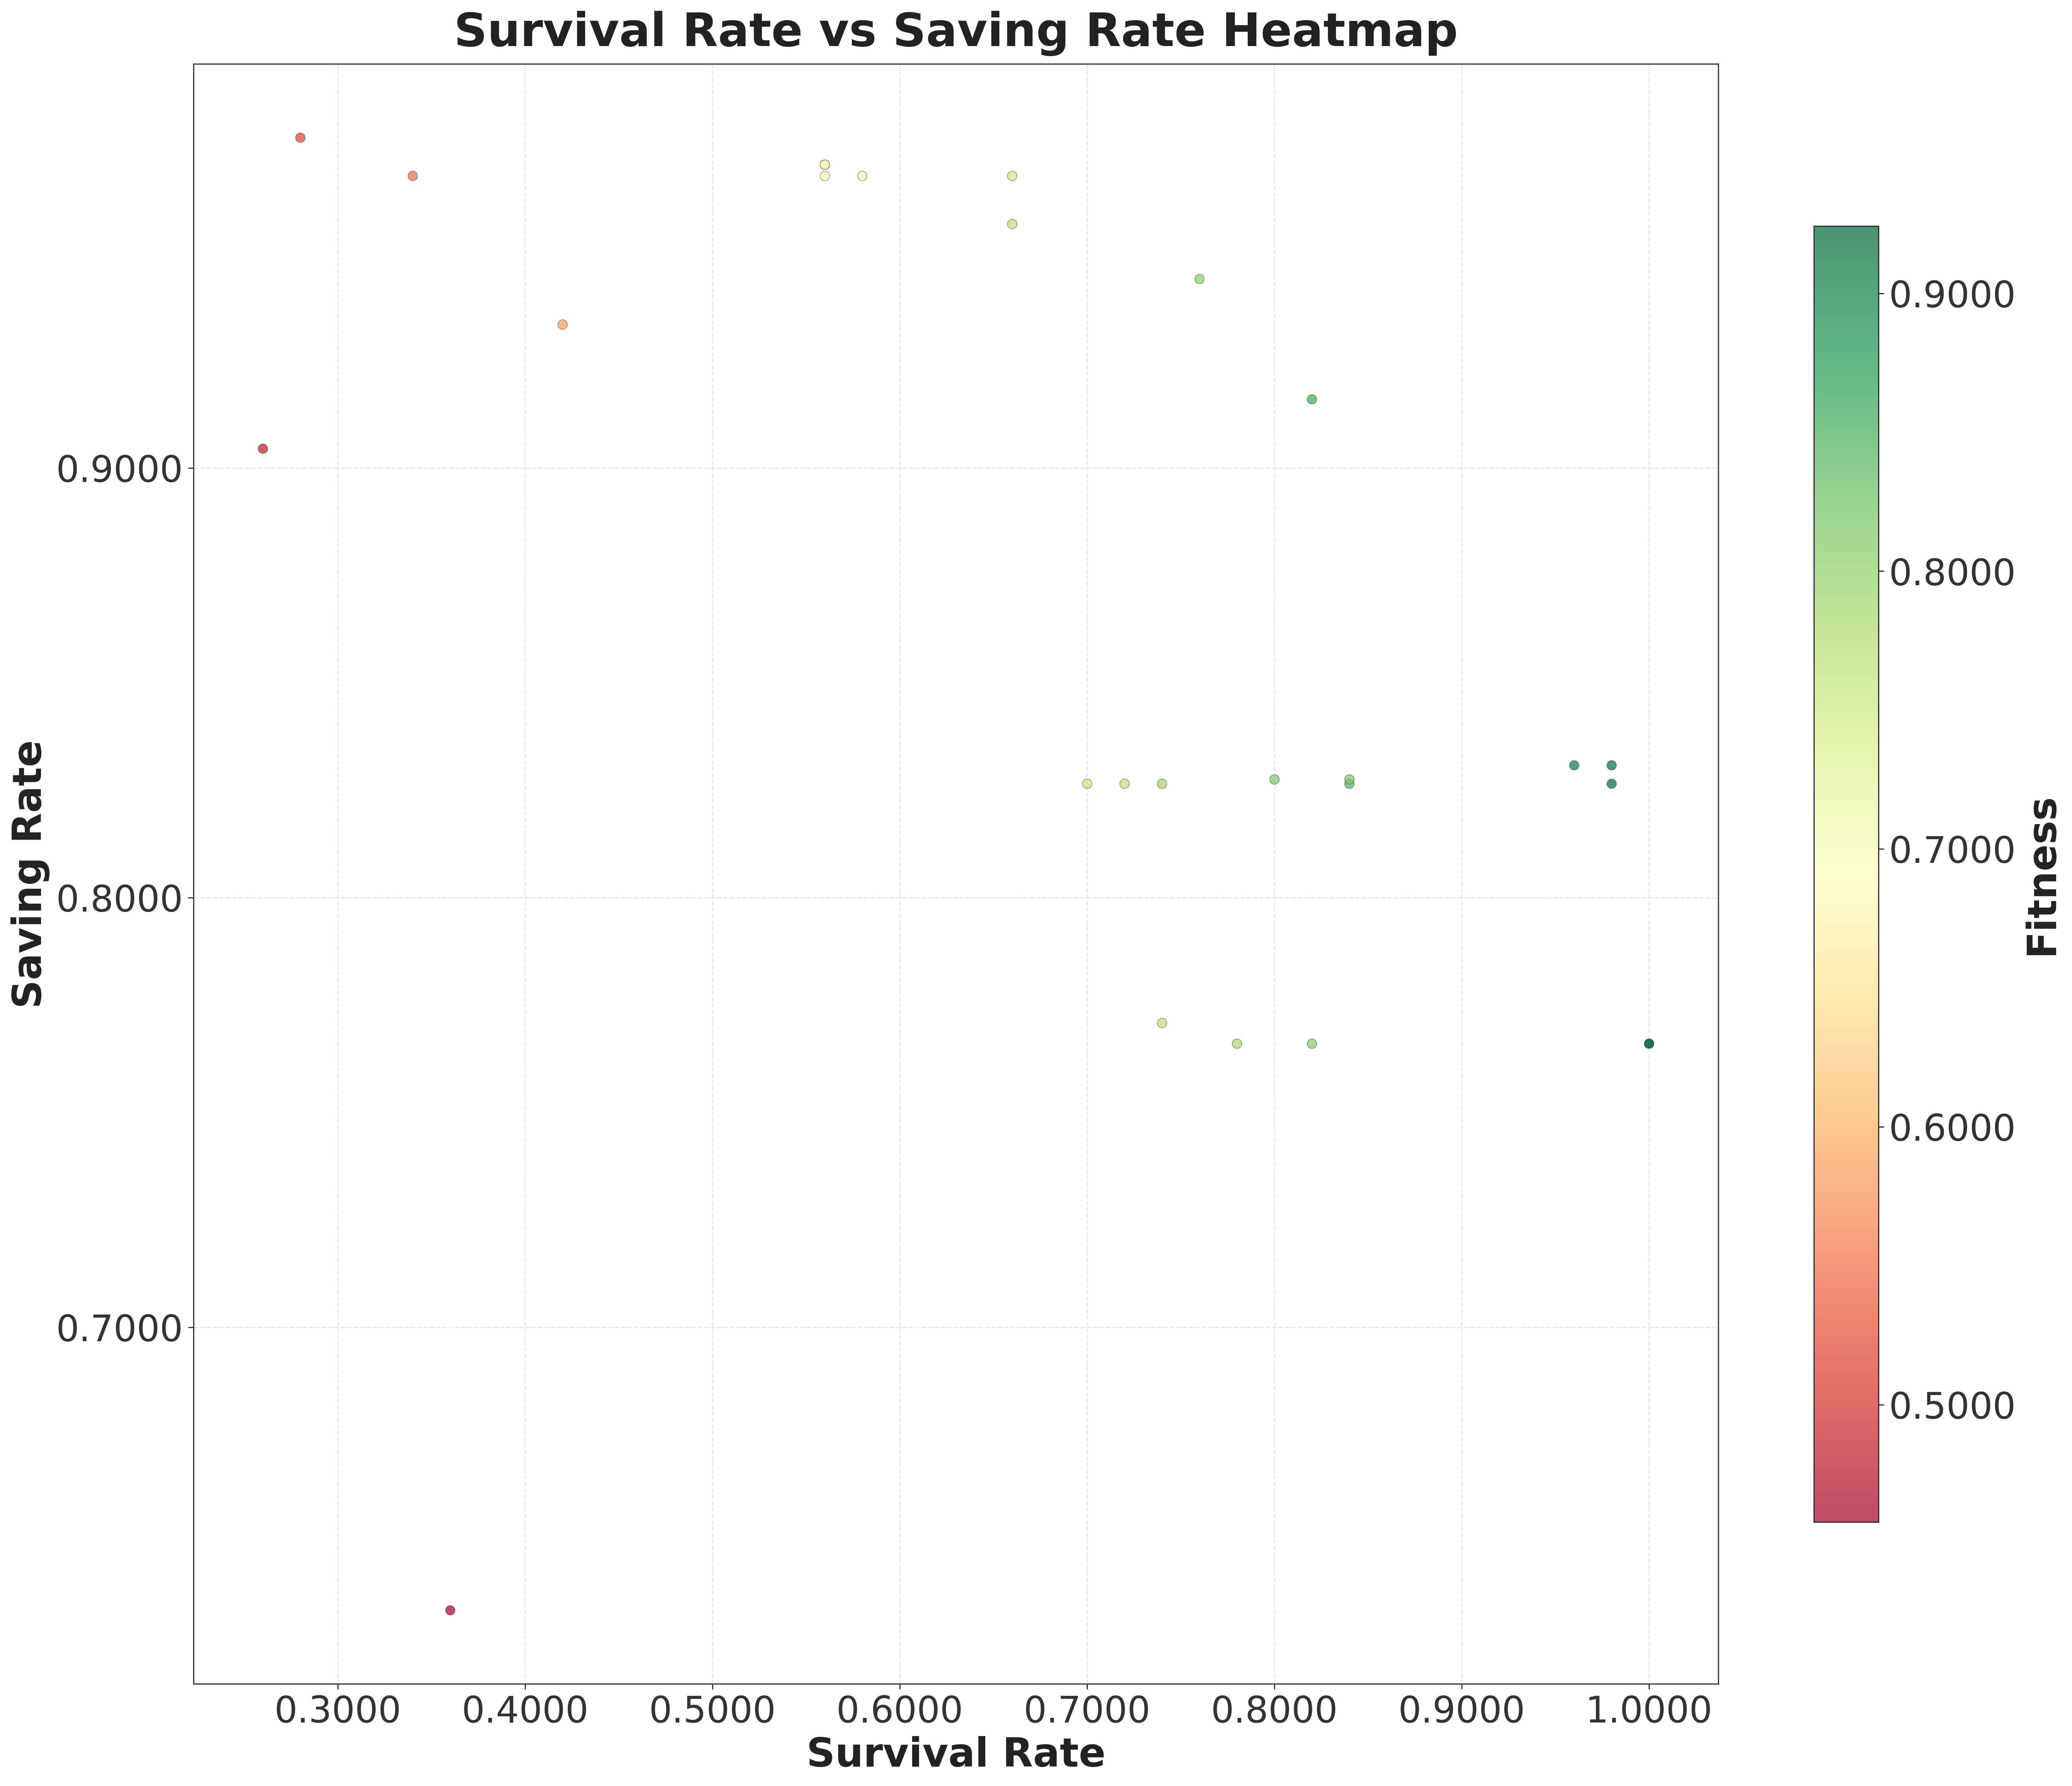
\includegraphics[width=0.42\textwidth]{../plots/plot_05_survival_rate_vs_saving_rate_heatmap.png}
\caption{Survival Rate vs Saving Rate Heatmap}
\label{fig:heat_surv_saving}
\end{figure}

The heatmap in Fig. \ref{fig:heat_surv_saving} reveals the dense clustering of evaluated policies regarding Survival versus Savings. The intense concentration in the upper-right quadrant visually confirms the EA's success in finding optimal points. Notably, there is a void in the extreme top-right corner (1.0 Survival, 1.0 Savings), mathematically proving that zero-cost survival is impossible in this environment. The distinct clusters also demonstrate that the algorithm frequently encounters a sharp Pareto frontier: to push survival from 80\% to 90\%, the policy must disproportionately sacrifice budget. Furthermore, the red dots scattered in the lower-left region of the plot reveal an interesting phenomenon: excessive spending can actually backfire. If the budget is heavily drained by dumping too much food and probiotics into the pond, the unconsumed leftovers decay into pollutants. These pollutants then transform into environmental hazards that harm the fish, leading to a lower survival rate despite the high resource expenditure.


\begin{figure}[H]
\centering
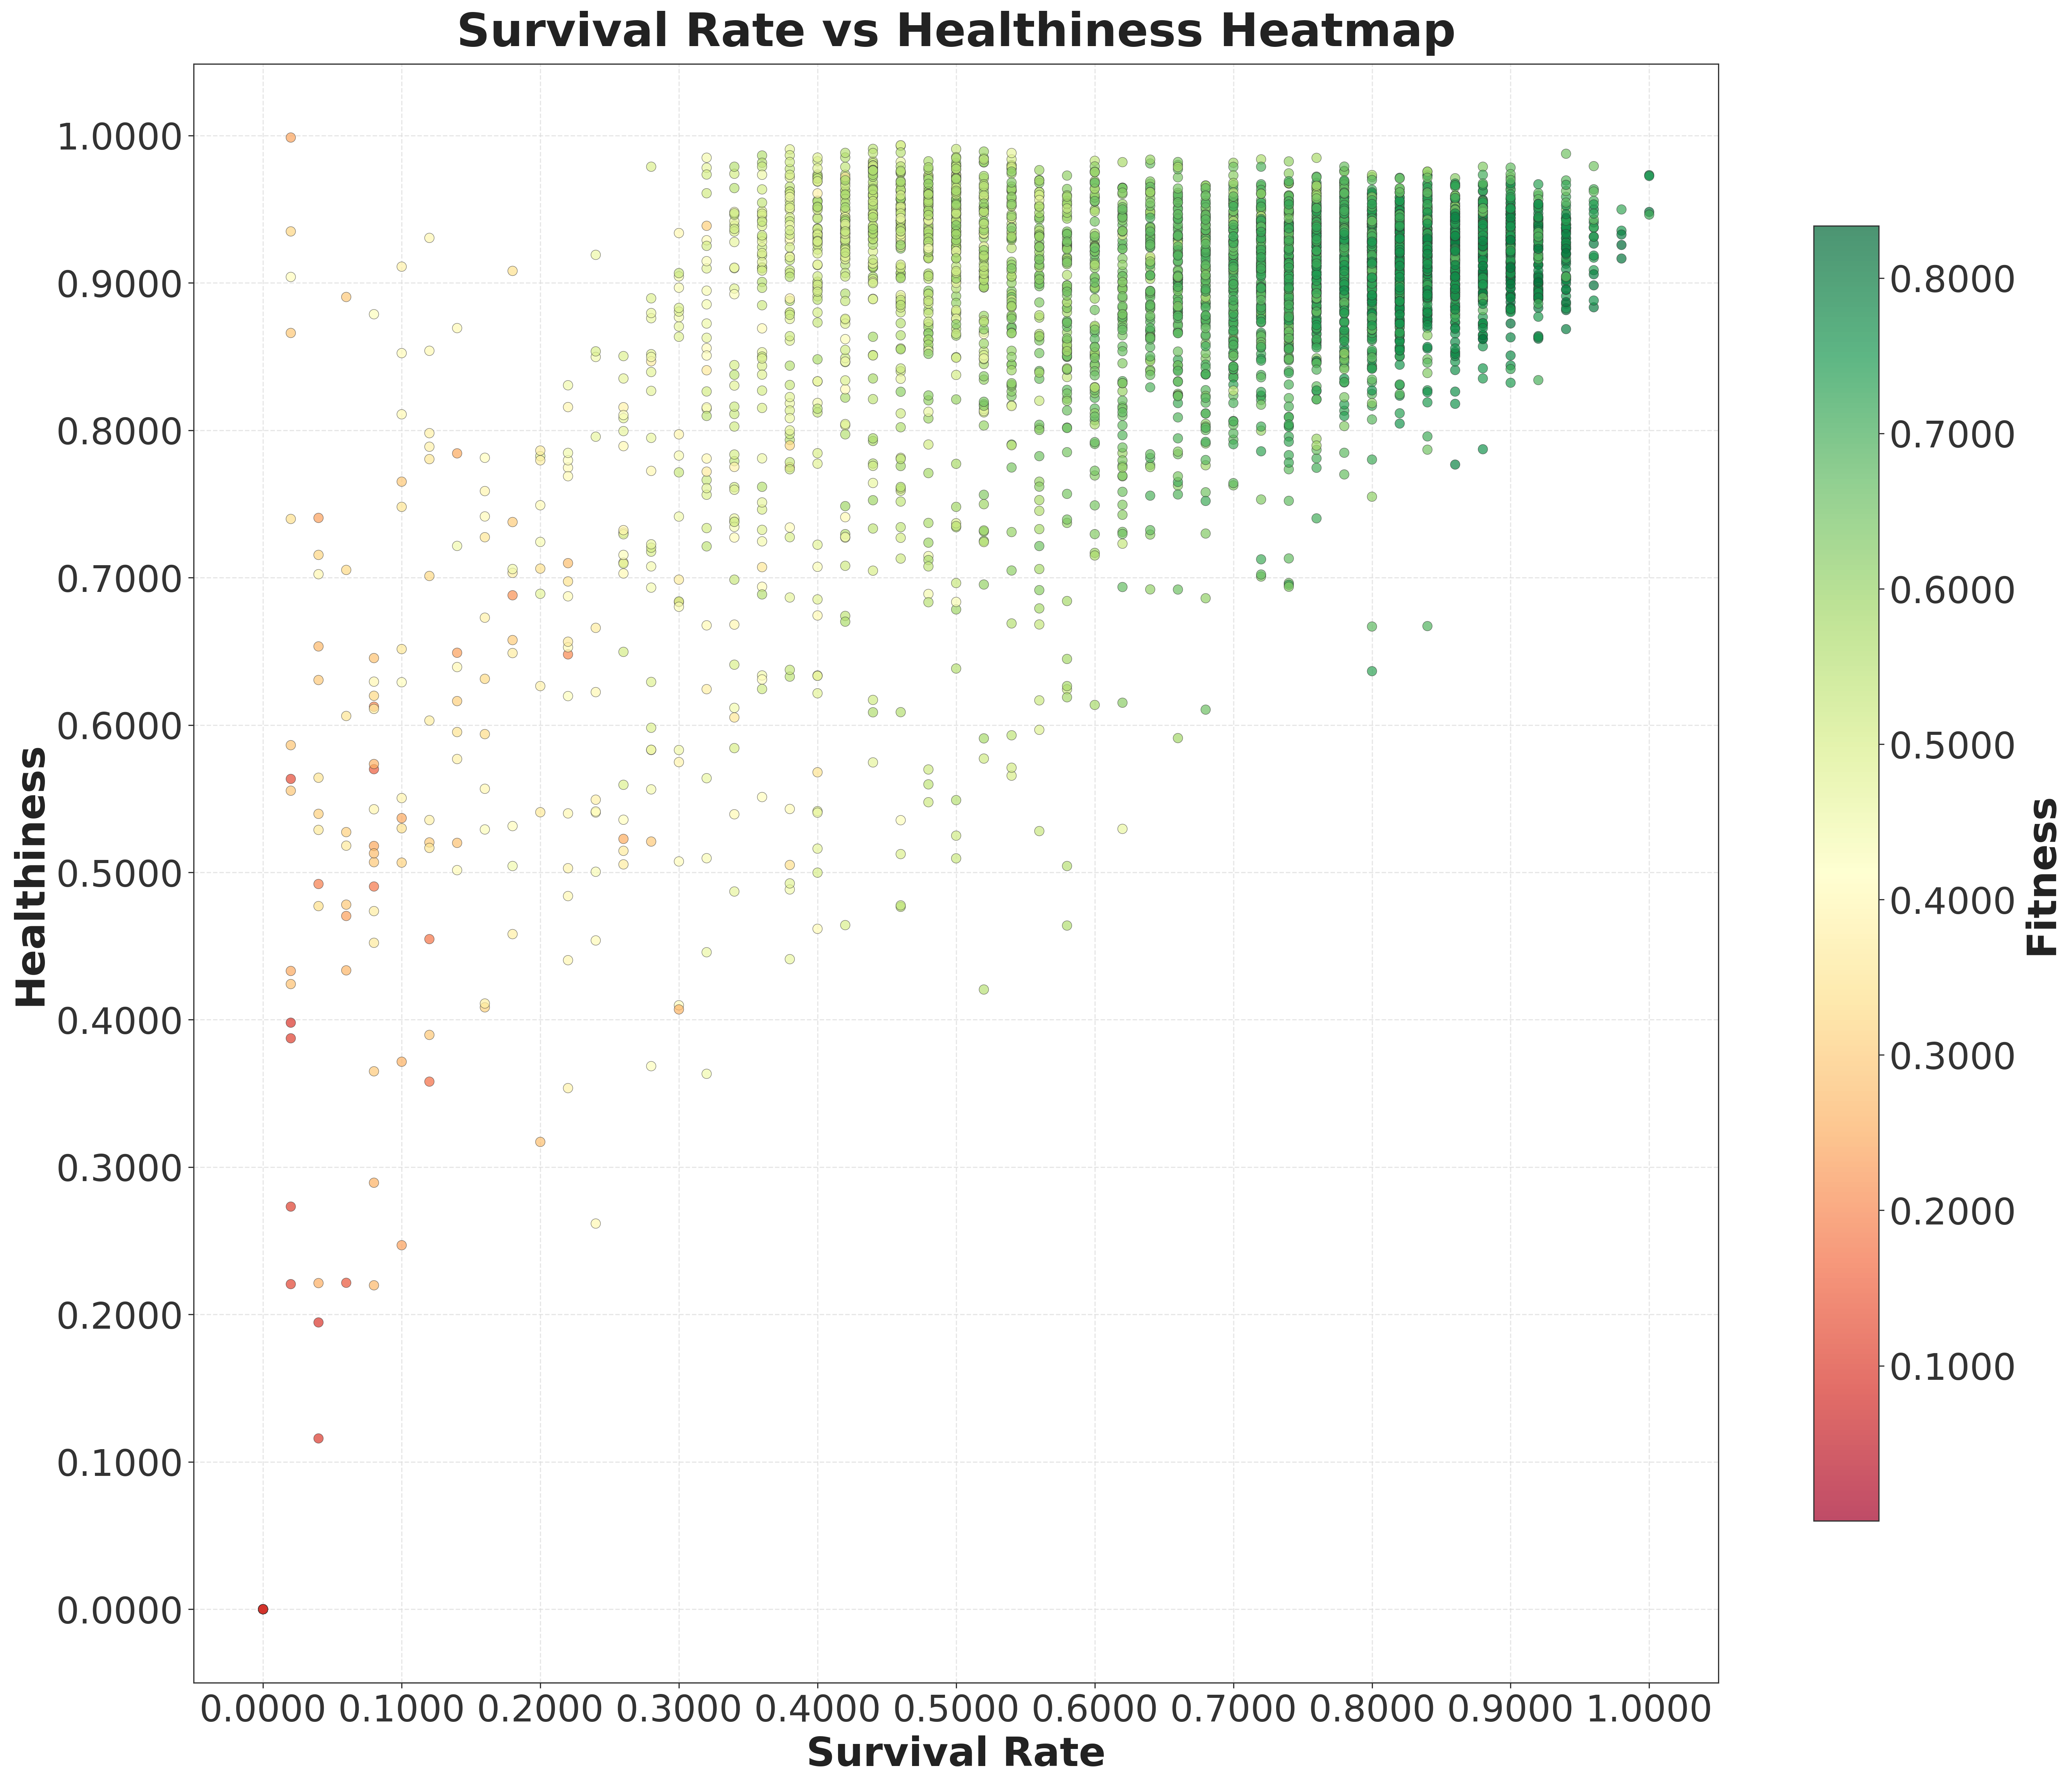
\includegraphics[width=0.42\textwidth]{../plots/plot_06_survival_rate_vs_healthiness_heatmap.png}
\caption{Survival Rate vs Healthiness Heatmap}
\label{fig:heat_surv_health}
\end{figure}

Fig. \ref{fig:heat_surv_health} illustrates the strong positive correlation between Survival Rate and Healthiness. The dense, diagonal clustering indicates these two metrics are highly collaborative rather than strictly competitive. Policies that successfully mitigate environmental hazards (like NH3 and parasites) and provide adequate nutrition naturally result in both higher survival numbers and higher average internal physiological scores for survivors.


\begin{figure}[H]
\centering
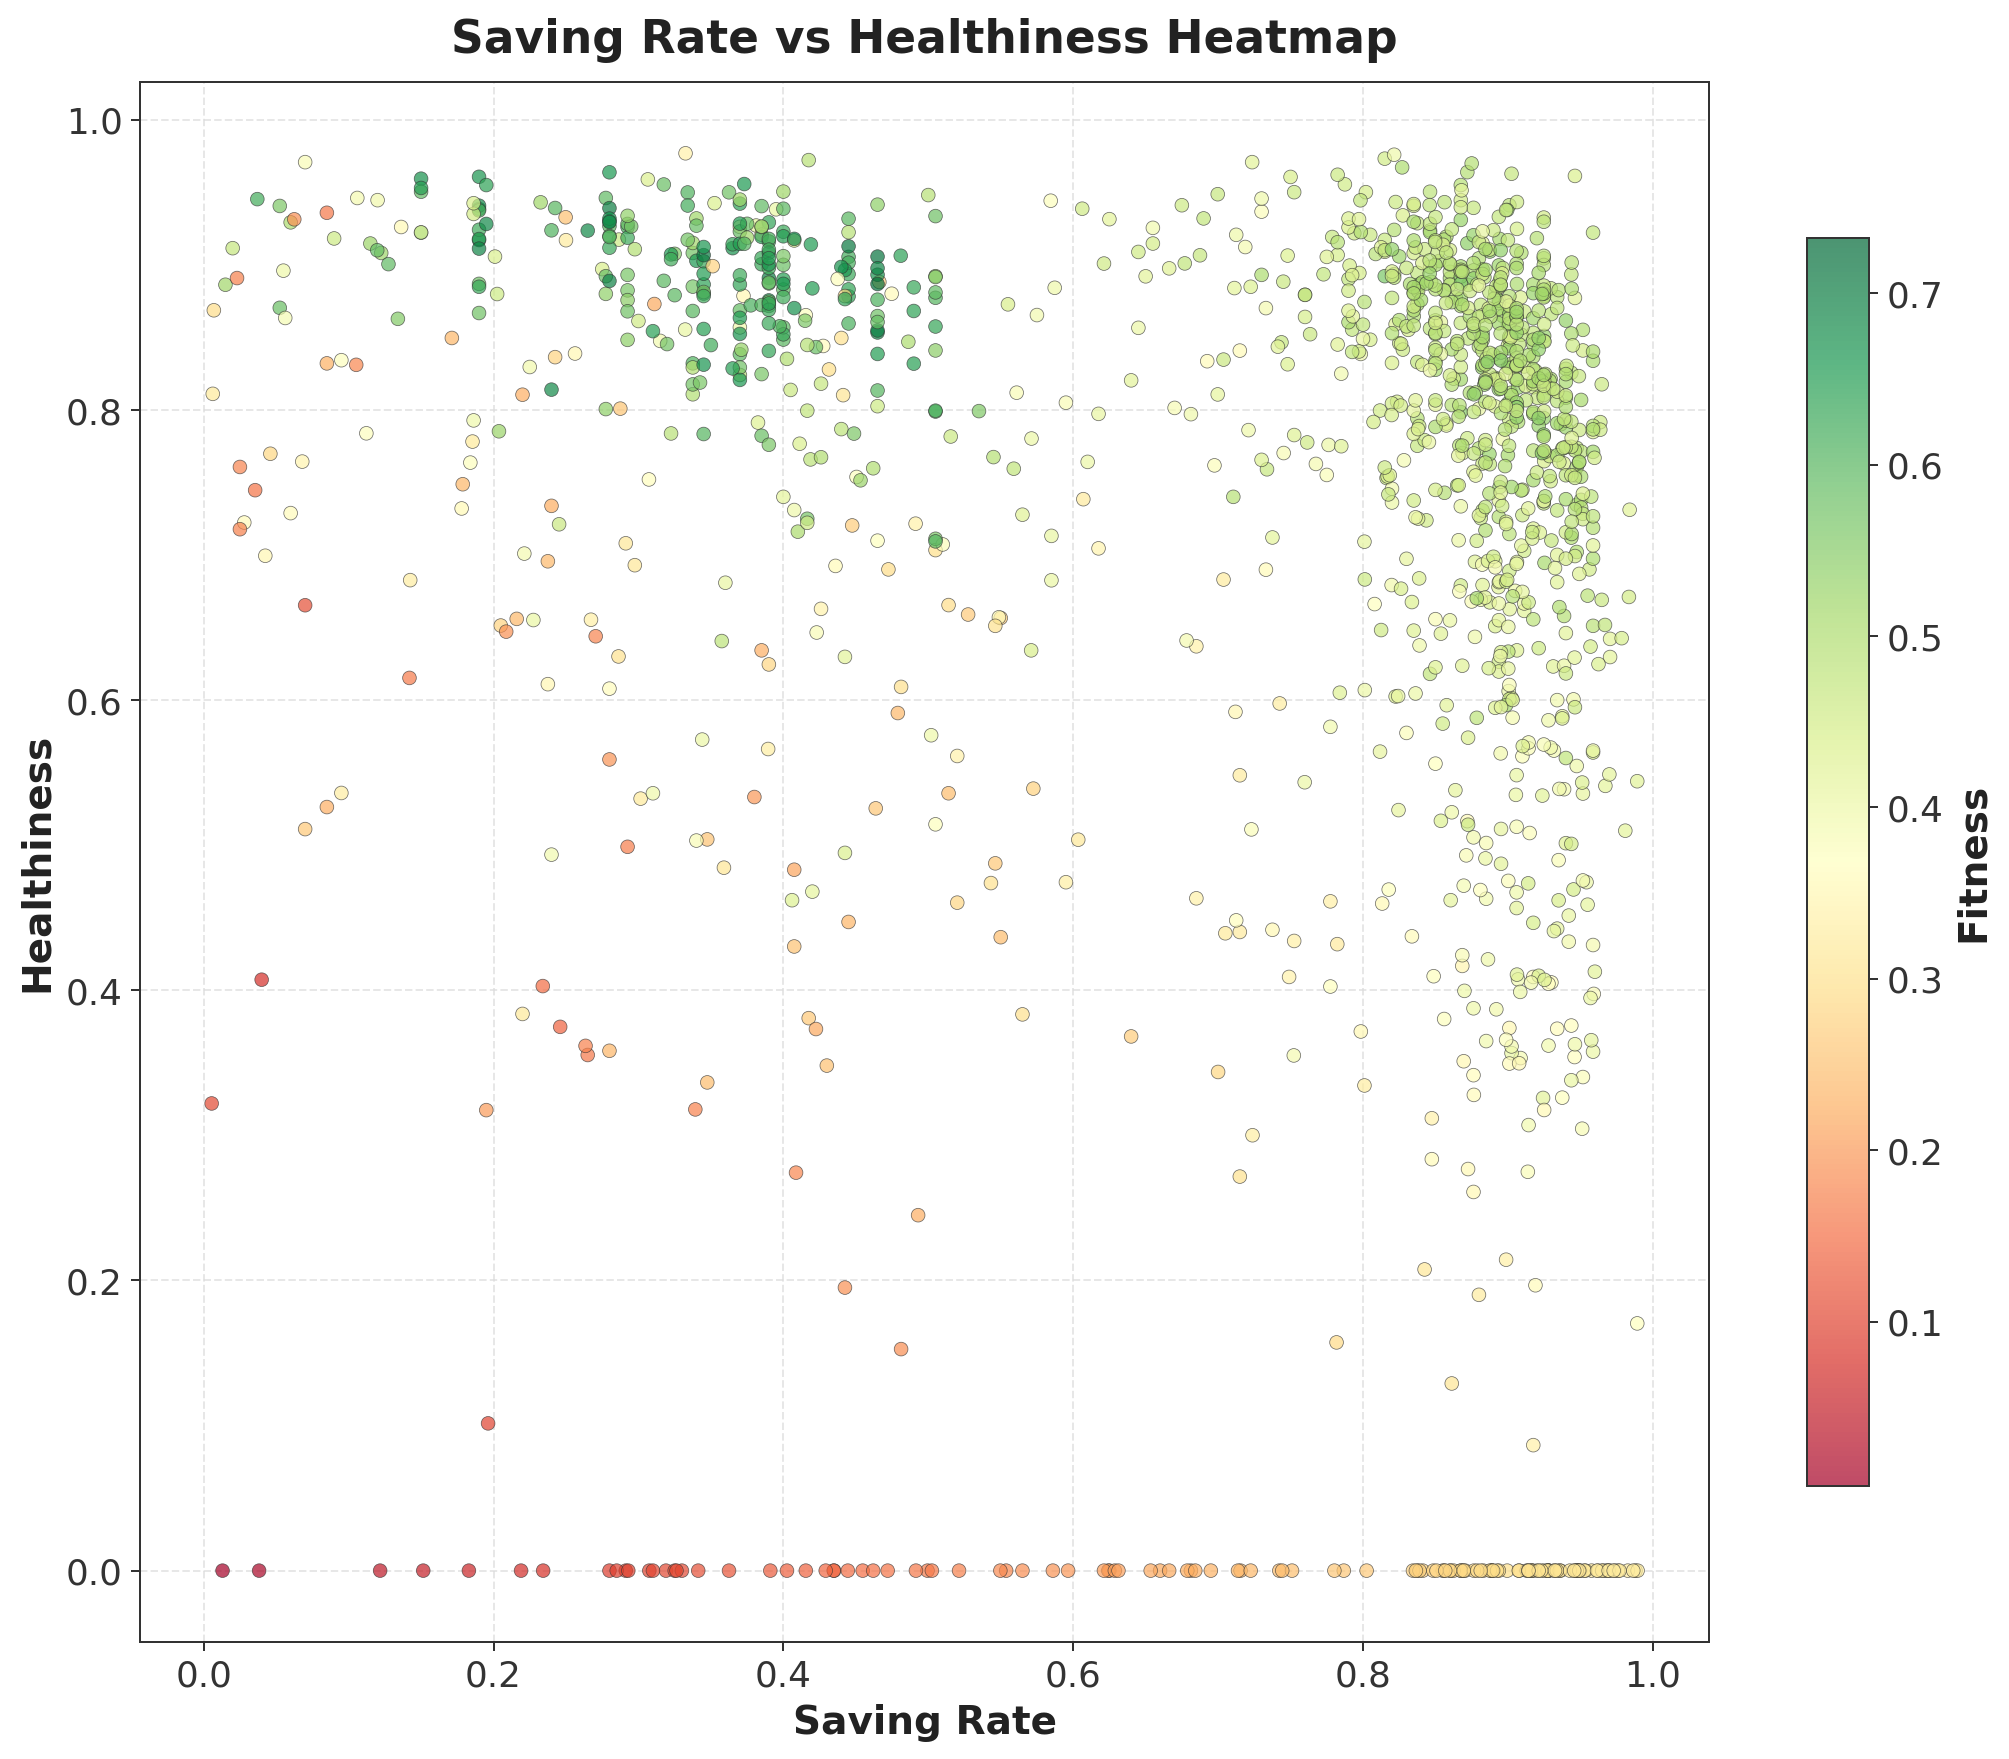
\includegraphics[width=0.42\textwidth]{../plots/plot_07_saving_rate_vs_healthiness_heatmap.png}
\caption{Saving Rate vs Healthiness Heatmap}
\label{fig:heat_saving_health}
\end{figure}

Given the intrinsic correlation between Survival Rate and Healthiness, Fig. \ref{fig:heat_saving_health} illustrates a complex, non-linear relationship characterized by substantial dispersion. The observed variance suggests that suboptimal resource allocation depletes financial reserves without improving Healthiness. Conversely, precisely optimized delivery schedules maintain high health standards while preserving economic efficiency. Consistent with trends observed in survival metrics, the results highlight an overspending backfire effect; excessive resource supplementation fosters pollutant accumulation and water quality degradation, thereby compromising fish immunity despite high capital investment.

Fig. \ref{fig:pop_dist} (located in Appendix) illustrates a dramatic shift from early-generation failures,dominated by over budget and all dead outcomes, to consistent success. By Generation 20, over 80\% of policies reached the OK status, visually confirming the robustness of the genetic convergence across all timelines. Notably, all generated policies were theoretically viable, as evidenced by zero Reject cases (Reject status is a pre-calculated early termination that automatically discards a genotype if its hard-coded parameters mathematically exceed the maximum budget).

As illustrated in Fig. \ref{fig:champ_comp} (Appendix), the ten timeline champions exhibit notable performance variance, with fitness scores spanning from 0.7498 to 0.8158. The lowest-scoring champion (Timeline 3) achieved the highest Saving Rate, while Timeline 9 maintained average fitness despite having the lowest savings. This non-linear relationship confirms that stochastic environmental luck, such as randomized hazard placement, heavily influences individual evaluations. Consequently, the robust champion average of approximately 0.7885 represents a more realistic optimization than any single stochastic peak.

Table \ref{tab:champ_tl10} details the TL-10 Champion's metrics and genotype. Achieving a 94\% survival rate and 0.8158 fitness for only \$208.50, the policy reveals a non-intuitive emergent strategy: completely abandoning expensive probiotics. Instead, it maximizes health with abundant nutrition and spatial logistics, demonstrating the EA's ability to discover synergistic, cost-effective environmental management solutions over chemical intervention.

\begin{table}[H]
\centering
\caption{Detailed Metrics and Genotype of the TL-10 Champion}
\label{tab:champ_tl10}
\resizebox{\linewidth}{!}{%
\begin{tabular}{|l|r|}
\hline
\textbf{Metric} & \textbf{Value} \\ \hline
Fitness & 0.8158 \\ \hline
Survival Rate & 0.9400 \\ \hline
Saving Rate & 0.5830 \\ \hline
Healthiness & 0.8869 \\ \hline
Cost & \$208.50 \\ \hline
Alive/Initial & 47/50 \\ \hline
Initial Fish & 50 \\ \hline
\end{tabular}%
\hspace{0.2cm}%
\begin{tabular}{|l|r|}
\hline
\textbf{Genotype} & \textbf{Value} \\ \hline
Food Interval & 5 h \\ \hline
Food Quantity & 10 pellets \\ \hline
Food Location & Random \\ \hline
Prob. Interval & 36 h \\ \hline
Prob. Quantity & 0 pellets \\ \hline
Prob. Location & Random \\ \hline
O2 Interval & 17 h \\ \hline
O2 Duration & 1 h \\ \hline
O2 Location & Random \\ \hline
\end{tabular}%
}
\end{table}

\section{Discussion, Conclusion, and Future Work}

\subsection{Discussion}
The EA successfully navigated a stochastic fitness landscape to optimize Largemouth Bass aquaculture, rapidly overcoming massive early-generation failures (``All-Dead'' and ``Over-Budget'' statuses). By employing a multi-objective fitness function to manage the underlying Particle Swarm Optimization (PSO) engine, the EA successfully balanced biological welfare with economic constraints.

Consequently, it discovered non-intuitive, highly effective strategies that challenge conventional management. Specifically, it learned to scatter food randomly to prevent localized ammonia spikes and applied probiotics as sparse immunity bumps rather than daily supplements. Furthermore, it aggressively restricted oxygen pumping to just one hour by exploiting the PSO swarm's natural ability to dynamically swim away from hypoxic dead zones.

\subsection{Conclusion}
AquaOptima successfully integrates an Evolutionary Algorithm (EA) manager with a Particle Swarm Optimization (PSO) engine for autonomous aquaculture management. By modeling Largemouth Bass as PSO agents with dynamic physiological needs, the system accurately simulates the reactive and chaotic nature of aquaculture. We conclude that this PSO interaction, where the swarm actively evades hazards and competes for localized resources, provides a realistic environment for testing policy robustness.

Operating within this environment, the EA effectively navigates inherent stochasticity, reliably mitigating biological hazards (e.g., cannibalism, ammonia, pathogens) while minimizing operational costs. Ultimately, the robust average champion fitness of 0.7885 represents a realistic optimization ``sweet spot,'' proving that proactive algorithmic management can successfully balance fish survival, internal health, and financial efficiency in unpredictable biological systems.

\subsection{Future Work}
Future iterations of AquaOptima will expand the simulation's biological scope beyond a static initial cohort. The first objective is to implement a secondary Evolutionary Algorithm to govern fish reproductive mechanics, allowing the swarm to dynamically breed and genetically adapt over extended, multi-season population cycles.

Furthermore, expanding into multi-species interactions introduces a new real-life dynamic. We plan to do so with polyculture dynamics, such as incorporating a bottom feeder species to naturally process decaying waste and fundamentally alter the toxic ammonia hazard loop.

Finally, future models will integrate more rigorous physical and environmental constraints. This includes the addition of dynamic weather patterns, simulated water currents, and seasonal temperature changes that directly influence the metabolic rates and behavioral responses of the fish.

\appendix[Supplementary Landscape Figures]
\label{app:landscape_figs}

\begin{sidewaysfigure}
\centering
\includegraphics[width=1.0\linewidth]{../plots/plot_11_pond_population_distribution.png}
\caption{Pond Population Distribution.}
\label{fig:pop_dist}
\end{sidewaysfigure}

\begin{sidewaysfigure}
\centering
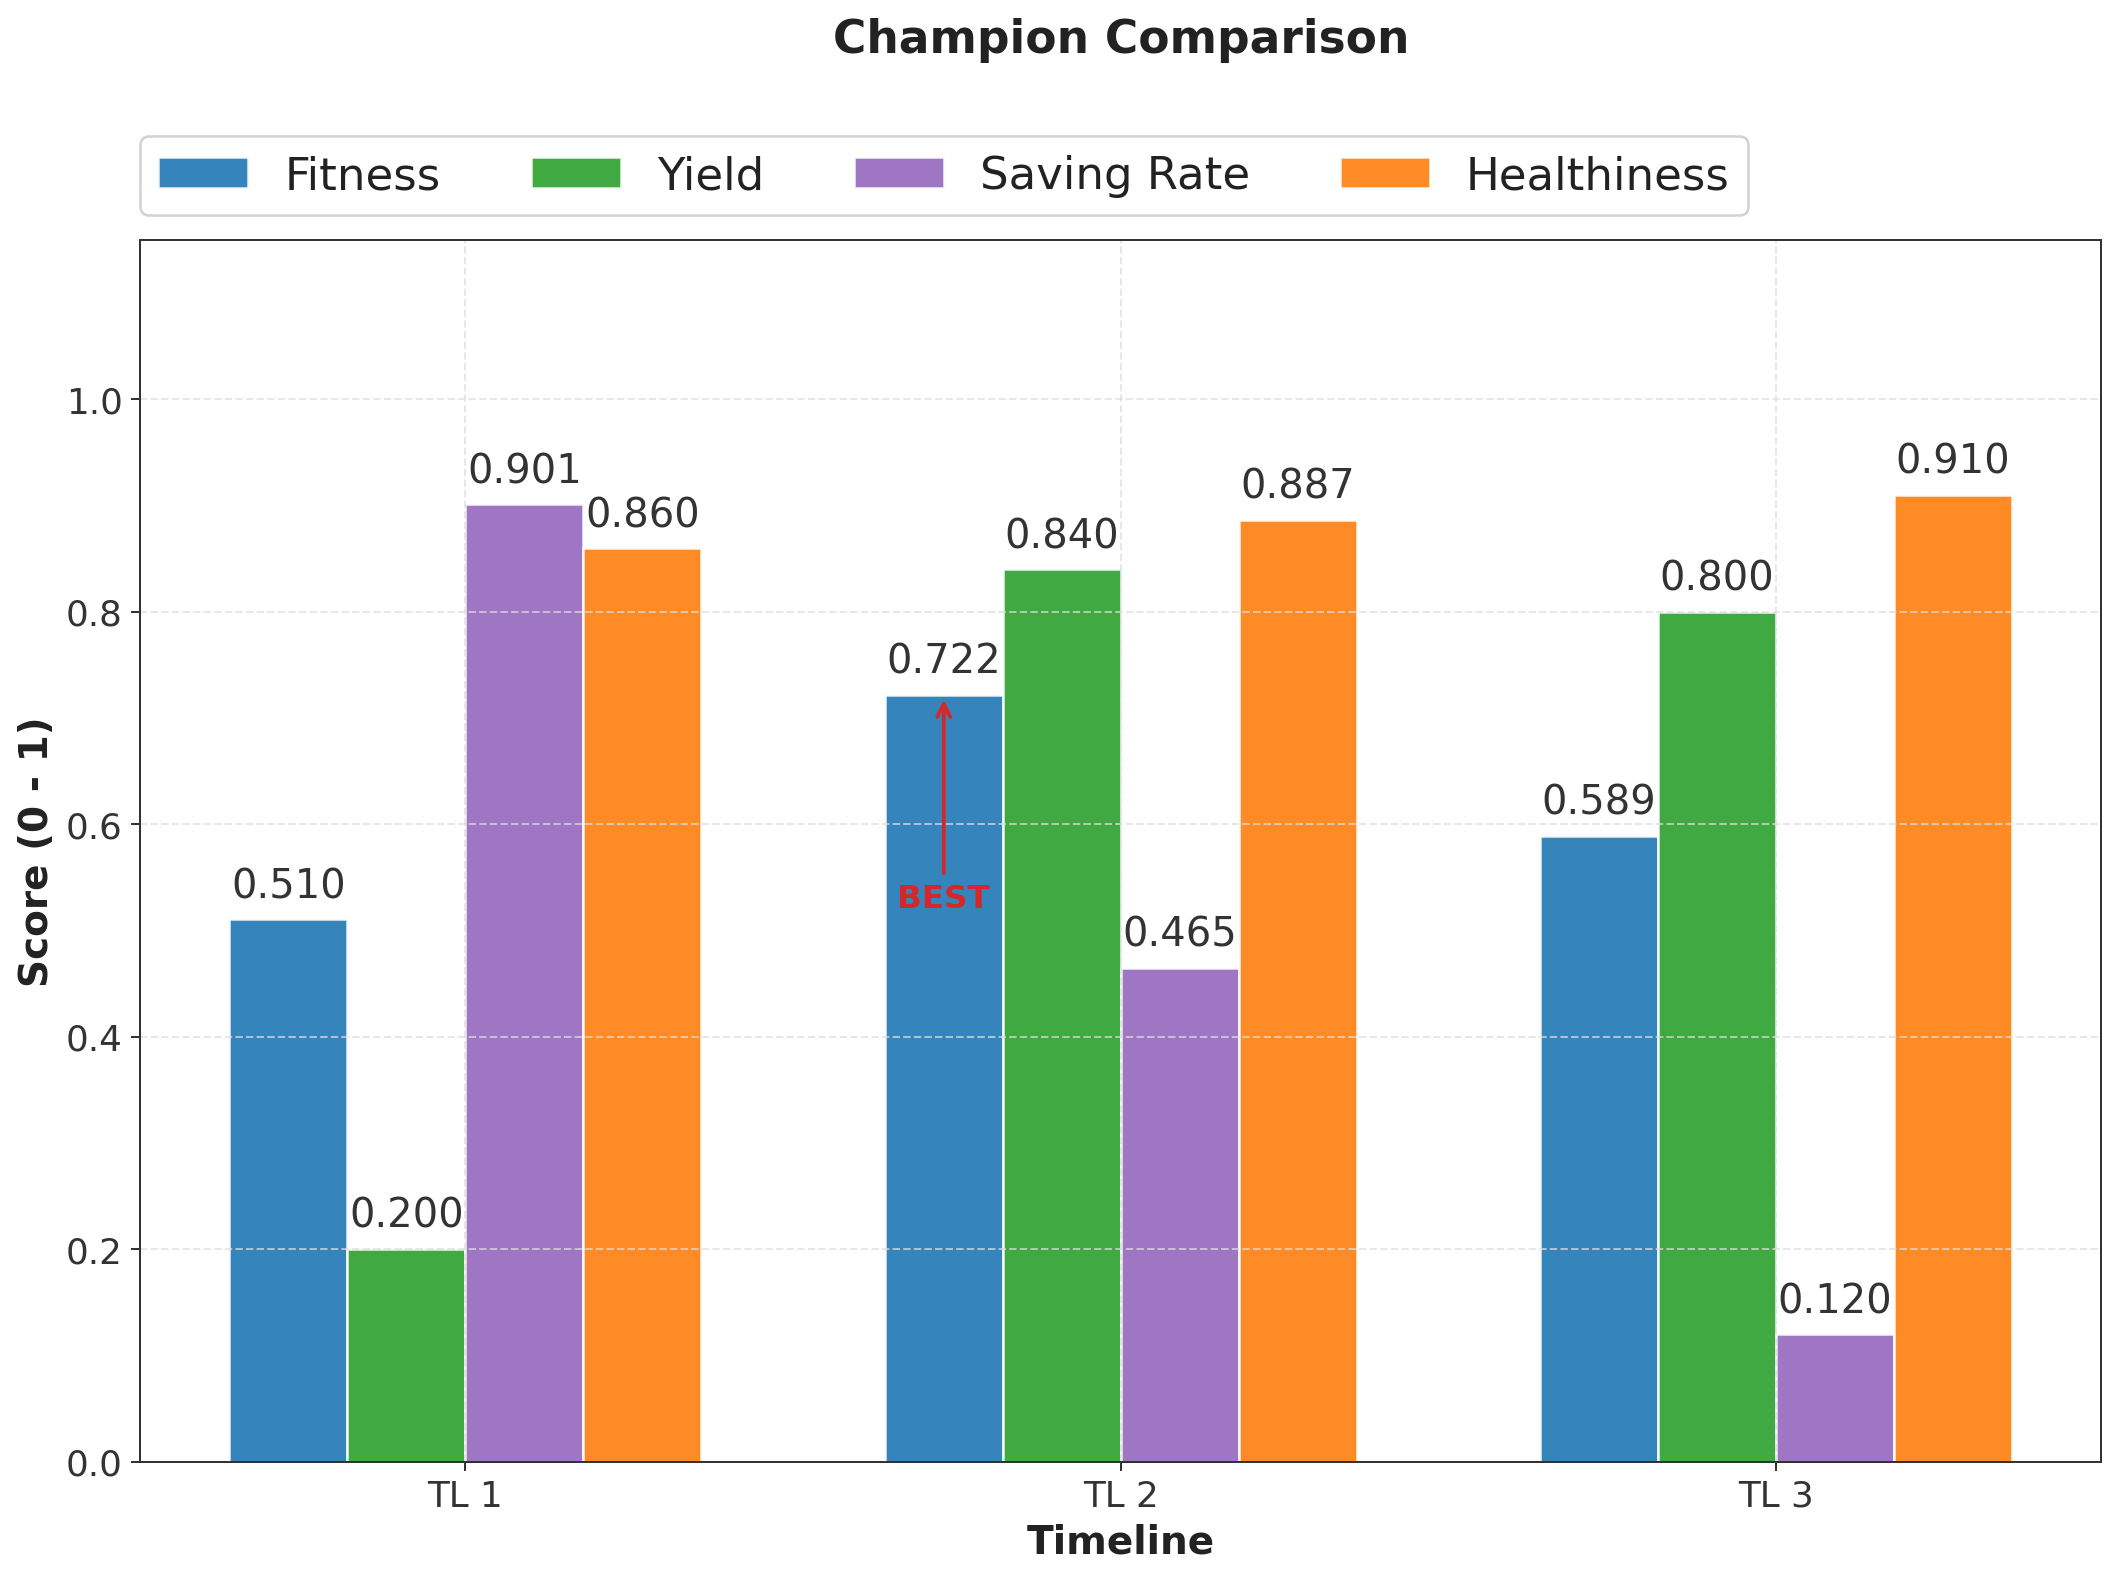
\includegraphics[width=1.0\linewidth]{../plots/plot_12_champion_comparison.png}
\caption{Champion Comparison.}
\label{fig:champ_comp}
\end{sidewaysfigure}

\clearpage
\begin{thebibliography}{00}

\bibitem{carrella2024} E. Carrella \textit{et al.}, ``Rejection sampling and agent-based models for data limited fisheries,'' \textit{Frontiers in Marine Science}, vol. 11, Jan. 2024, doi: 10.3389/fmars.2024.1243954.

\bibitem{urbanova2023} P. Urbanova, I. Koliada, P. Císař, and M. Železný, ``Agent Based Modeling of Fish Shoal Behavior,'' \textit{Lecture Notes in Computer Science}, pp. 3--13, 2023, doi: 10.1007/978-3-031-34960-7\_1.

\bibitem{hou2023} H. Hou, A. Ren, L. Yu, Z. Ma, Z. Yun, and Y. Liu, ``An Environmental Impact Assessment of Largemouth Bass (\textit{Micropterus salmoides}) Aquaculture in Hangzhou, China,'' \textit{Sustainability}, vol. 15, no. 16, pp. 12368--12368, Aug. 2023, doi: 10.3390/su151612368.

\bibitem{bowker2013} J. D. Bowker, D. Carty, J. T. Trushenski, M. P. Bowman, N. Wandelear, and M. D. Matthews, ``Controlling Mortality Caused by External Columnaris in Largemouth Bass and Bluegill with Chloramine-T or Hydrogen Peroxide,'' \textit{North American Journal of Aquaculture}, vol. 75, no. 3, pp. 342--351, Jul. 2013, doi: 10.1080/15222055.2013.783521.

\bibitem{tu2025} Y.-Y. Tu \textit{et al.}, ``A Comprehensive Investigation of Potential Bacterial Pathogens in Largemouth Bass (\textit{Micropterus salmoides}),'' \textit{Microorganisms}, vol. 13, no. 6, pp. 1413--1413, Jun. 2025, doi: 10.3390/microorganisms13061413.

\bibitem{wang2024} C. Wang \textit{et al.}, ``Multiple effects of dietary supplementation with \textit{Lactobacillus reuteri} and \textit{Bacillus subtilis} on the growth, immunity, and metabolism of largemouth bass (\textit{Micropterus salmoides}),'' \textit{Developmental \& Comparative Immunology}, vol. 160, p. 105241, Nov. 2024, doi: 10.1016/j.dci.2024.105241.

\bibitem{johnson1996} J. M. Johnson and D. M. Post, ``Morphological Constraints on Intracohort Cannibalism in Age-0 Largemouth Bass,'' \textit{Transactions of the American Fisheries Society}, vol. 125, no. 5, pp. 809--812, Sep. 1996, doi: 10.1577/1548-8659(1996)125\textless{}0809:MCOICI\textgreater{}2.3.CO;2.

\bibitem{kennedy1995} J. Kennedy and R. Eberhart, ``Particle swarm optimization,'' \textit{Proceedings of ICNN'95 - International Conference on Neural Networks}, vol. 4, pp. 1942--1948, 1995, doi: 10.1109/icnn.1995.488968.

\bibitem{tidwell1998} J. H. Tidwell, S. D. Coyle, and C. D. Webster, ``Effect of stocking density on growth and water quality for largemouth bass \textit{Micropterus salmoides} growout in ponds,'' \textit{Aquaculture}, vol. 145, pp. 213--223, 1998.

\bibitem{hinterding1995} R. Hinterding, ``Gaussian mutation and self-adaptation for numeric genetic algorithms,'' \textit{Proceedings of 1995 IEEE International Conference on Evolutionary Computation}, Perth, WA, Australia, 1995, pp. 384--389, doi: 10.1109/ICEC.1995.489178.

\bibitem{wang2025} B. Wang, H. Yang, H. Mao, and Q. Shi, ``Development and Testing of an Aquaculture Environmental Control System Based on Behavioral Stress Responses,'' \textit{Life}, vol. 15, no. 12, p. 1809, Nov. 2025, doi: 10.3390/life15121809.

\bibitem{derrac2011} J. Derrac, S. García, D. Molina, and F. Herrera, ``A practical tutorial on the use of nonparametric statistical tests as a methodology for comparing evolutionary and swarm intelligence algorithms,'' \textit{Swarm and Evolutionary Computation}, vol. 1, no. 1, pp. 3--18, Mar. 2011, doi: 10.1016/j.swevo.2011.02.002.

\end{thebibliography}

\end{document}